\documentclass[11pt]{article}

% Change "review" to "final" to generate the final (sometimes called camera-ready) version.
% Change to "preprint" to generate a non-anonymous version with page numbers.
\usepackage[review]{acl}

% Standard package includes
\usepackage{times}
\usepackage{latexsym}

% For proper rendering and hyphenation of words containing Latin characters (including in bib files)
\usepackage[T1]{fontenc}
% For Vietnamese characters
% \usepackage[T5]{fontenc}
% See https://www.latex-project.org/help/documentation/encguide.pdf for other character sets

% This assumes your files are encoded as UTF8
\usepackage[utf8]{inputenc}

% This is not strictly necessary, and may be commented out,
% but it will improve the layout of the manuscript,
% and will typically save some space.
\usepackage{microtype}

% This is also not strictly necessary, and may be commented out.
% However, it will improve the aesthetics of text in
% the typewriter font.
\usepackage{inconsolata}

%Including images in your LaTeX document requires adding
%additional package(s)
\usepackage{graphicx}
\usepackage{booktabs}
\usepackage{enumitem}
\usepackage{amsmath}
\usepackage{subcaption}
\usepackage{xcolor}
\usepackage{cleveref}
\usepackage{fancyvrb}
\usepackage{stfloats}

\usepackage{amssymb}
\usepackage{fvextra}
\usepackage[table,dvipsnames]{xcolor}

% \placeholder marks cells / sentences that will be filled in once the
% current full-benchmark run + ablation runs complete. Compiles in red
% so unfilled cells stand out at proof-read time.
\newcommand{\placeholder}{\textcolor{red}{\textsf{[TBD]}}}
% If the title and author information does not fit in the area allocated, uncomment the following
%
%\setlength\titlebox{<dim>}
%
% and set <dim> to something 5cm or larger.

\title{Plan2Map: A Multimodal Benchmark for Document-Grounded Geospatial Boundary Reconstruction}

% \title{Plan2Map: A Multimodal Benchmark for Automatic Digitisation of UK Planning Records}

% Author information can be set in various styles:
% For several authors from the same institution:
% \author{Author 1 \and ... \and Author n \\
%         Address line \\ ... \\ Address line}
% if the names do not fit well on one line use
%         Author 1 \\ {\bf Author 2} \\ ... \\ {\bf Author n} \\
% For authors from different institutions:
% \author{Author 1 \\ Address line \\  ... \\ Address line
%         \And  ... \And
%         Author n \\ Address line \\ ... \\ Address line}
% To start a separate ``row'' of authors use \AND, as in
% \author{Author 1 \\ Address line \\  ... \\ Address line
%         \AND
%         Author 2 \\ Address line \\ ... \\ Address line \And
%         Author 3 \\ Address line \\ ... \\ Address line}

\author{First Author \\
  Affiliation / Address line 1 \\
  Affiliation / Address line 2 \\
  Affiliation / Address line 3 \\
  \texttt{email@domain} \\\And
  Second Author \\
  Affiliation / Address line 1 \\
  Affiliation / Address line 2 \\
  Affiliation / Address line 3 \\
  \texttt{email@domain} \\}

%\author{
%  \textbf{First Author\textsuperscript{1}},
%  \textbf{Second Author\textsuperscript{1,2}},
%  \textbf{Third T. Author\textsuperscript{1}},
%  \textbf{Fourth Author\textsuperscript{1}},
%\\
%  \textbf{Fifth Author\textsuperscript{1,2}},
%  \textbf{Sixth Author\textsuperscript{1}},
%  \textbf{Seventh Author\textsuperscript{1}},
%  \textbf{Eighth Author \textsuperscript{1,2,3,4}},
%\\
%  \textbf{Ninth Author\textsuperscript{1}},
%  \textbf{Tenth Author\textsuperscript{1}},
%  \textbf{Eleventh E. Author\textsuperscript{1,2,3,4,5}},
%  \textbf{Twelfth Author\textsuperscript{1}},
%\\
%  \textbf{Thirteenth Author\textsuperscript{3}},
%  \textbf{Fourteenth F. Author\textsuperscript{2,4}},
%  \textbf{Fifteenth Author\textsuperscript{1}},
%  \textbf{Sixteenth Author\textsuperscript{1}},
%\\
%  \textbf{Seventeenth S. Author\textsuperscript{4,5}},
%  \textbf{Eighteenth Author\textsuperscript{3,4}},
%  \textbf{Nineteenth N. Author\textsuperscript{2,5}},
%  \textbf{Twentieth Author\textsuperscript{1}}
%\\
%\\
%  \textsuperscript{1}Affiliation 1,
%  \textsuperscript{2}Affiliation 2,
%  \textsuperscript{3}Affiliation 3,
%  \textsuperscript{4}Affiliation 4,
%  \textsuperscript{5}Affiliation 5
%\\
%  \small{
%    \textbf{Correspondence:} \href{mailto:email@domain}{email@domain}
%  }
%}

\begin{document}
\maketitle

% ITS PLACES BEFORE ABSTRACT, BUT OVERWRITTING THE TEXT
% \begin{center}
%     \centering
%     \captionsetup{type=figure}
%     \includegraphics[
%     width=\textwidth,
%     trim={6.9cm 4.7cm 7.4cm 7.1cm},   
%     clip                
%     ]{teaser_fig.pdf}
%     \caption{\textbf{Plan2Map}}
% \end{center}


   

\rowcolors{2}{gray!15}{white}      % every even row light gray

\begin{abstract}
Planning records define restrictions over geographic areas, but source documents often provide only indirect spatial evidence rather than ready-to-use geospatial boundaries. We introduce \textbf{Plan2Map}, a multimodal benchmark for document-grounded geospatial boundary reconstruction from public planning records. Given only a source planning document, systems must reconstruct a valid geospatial boundary from notice text, schedules, map plates, labels, and boundary annotations. We propose \textbf{GeoPlanAgent}, a document-grounded, geospatial-tool-in-the-loop system that decomposes the task into evidence extraction, localisation, map registration, boundary segmentation, projection, and verification. On 208 cases, GeoPlanAgent achieves 0.690 mean IoU and 0.895 median IoU, with 74.5\% of predictions above 0.5 IoU. Diagnostic analysis reveals a strongly bimodal success pattern and identifies localisation and boundary extraction as the dominant bottlenecks. Plan2Map provides a concrete testbed for multimodal geospatial reconstruction from public planning records.
\end{abstract}

\section{Introduction}
\label{section:intro}

\begin{figure*}[t]
    \centering
    % \captionsetup{type=figure}
    \vspace{-15mm}
    \resizebox{0.76\textwidth}{!}{
    % \includegraphics[
    %      width=13.5cm,
    %      height=4.2cm,
    %     trim={6.9cm 5.64cm 7.7cm 7.1cm}, % Crop order: left bottom right top
    %     clip % Apply the crop
    % ]{teaser_fig.pdf}
    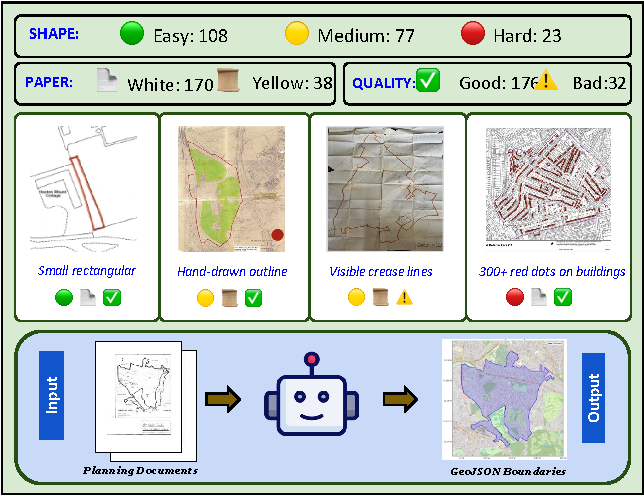
\includegraphics[]{fig/teaser.pdf}
    }
    \caption{\textbf{Plan2Map overview:} Given a source planning document, a system need to reconstruct the corresponding geospatial boundary.}
    % .Given a long planning document, our GeoPlan Agent, digitalised the required geospatial boundary
    \label{fig:teaser}
\end{figure*}

Planning records often answer a spatial question: \emph{which area is subject to a particular rule}? For UK Article~4 Directions \citep{planningdata2026article4direction}, this area is typically described through a legal notice and an accompanying map rather than provided as a machine-readable boundary. The operational form of these records is a concrete geospatial boundary: a planning system must know whether a site or application falls inside an affected area, compare the restriction with other planning datasets, and audit or update the record over time. In the source documents, however, this boundary is rarely available as a ready-to-use geospatial object. It is usually communicated indirectly through notice text, legal schedules, scanned or embedded map plates, map labels, coloured or hatched regions, and boundary annotations. Recovering the boundary is therefore not simply a matter of extracting a field from a document; it requires reconstructing a structured spatial object from distributed textual, visual, and geographic evidence.


This reconstruction problem is practically important for planning-record digitisation, where government and industry efforts such as the ``Extract initiative'' seek to convert legacy planning records into structured digital data \citep{govuk2025extract,colebourn2025extract}. Recent reviews of planning-application delays further underscore the need for efficient planning information flows \citep{weinstein2024UKgov,mhclg2026planningdelays}. Although public planning-data portals\footnote{https://www.planning.data.gov.uk/entity/?dataset=article-4-direction-area} may publish spatial records for some Article~4 Directions, including GeoJSON geometries, these records should be understood as evaluation references rather than task inputs: in our setting, the system is given only the source planning document. The challenge is to recover the boundary that a human would infer from the document itself, not to retrieve or copy a pre-existing geometry.



% Without machine-actionable boundary data, authorities and downstream users must manually interpret documents, maps, and boundary annotations to reconstruct the affected area, a slow and error-prone process that does not scale across local-authority archives.

We frame this setting as \emph{document-grounded geospatial boundary reconstruction} and introduce \textbf{Plan2Map}, a multimodal benchmark for reconstructing machine-readable geospatial boundaries from planning documents. As demonstrated in Fig.\ref{fig:teaser}, each example pairs a UK Article~4 Direction source document with a verified reference geometry. At evaluation time, the only case-specific input is the source planning document: the reference GeoJSON is held out for scoring, while systems may use declared public geospatial resources such as gazetteers and basemaps. Unlike standard document-understanding tasks that return textual answers, tables, or labels, Plan2Map requires a system to transform dispersed textual and visual evidence into an externally verifiable geospatial object.


This task is challenging because the boundary is not stated in machine-readable coordinates. A system must move from legal-document evidence to geographic grounding and finally to polygon reconstruction, while handling heterogeneous PDFs containing scanned pages, embedded maps, ambiguous boundary symbols, and textual qualifications. These properties make Plan2Map a stress test for multimodal systems that must produce structured spatial outputs rather than textual responses alone. To establish a strong baseline, we propose \textbf{GeoPlanAgent}, a decomposition-based reference system for Plan2Map. GeoPlanAgent separates the problem into document reading, localization, map registration, boundary extraction, projection, and verification, allowing us to diagnose which stages limit current multimodal systems.
 
Our \textbf{main contributions} are: \textbf{(i)} We introduce \textbf{Plan2Map}, a public, manually reviewed benchmark for document-grounded geospatial boundary reconstruction, built from UK Article~4 source documents and verified boundary geometries; \textbf{(ii)} We define the associated task and evaluation protocol: given only the source planning document, a system must reconstruct a valid geospatial boundary, evaluated by geometric overlap, polygon F1, centroid error, valid-output rate, and cost; \textbf{(iii)} We propose \textbf{GeoPlanAgent}, a decomposition-based system that mirrors the task structure through reading, localization, map registration, boundary segmentation, projection, and verification; and \textbf{(iv)} We provide diagnostic analysis with direct VLM baselines, essential component ablations, and a failure taxonomy, showing that localization and boundary extraction are the dominant bottlenecks.


\section{Related Work}

\paragraph{Multimodal Document and Geospatial Reasoning.}

Recent work has made substantial progress on multimodal document understanding and geospatial reasoning, but these capabilities have mostly been evaluated in separate settings. Document-understanding benchmarks such as DocVQA test whether models can read document images and answer questions over text, layout, and visual structure, while LayoutLMv3 and Donut represent layout-aware and OCR-free approaches to document understanding \citep{mathew2021docvqa,huang2022layoutlmv3,kim2022donut}. Geospatial VQA and remote-sensing benchmarks such as RSVQA, EarthVQA, GeoChat, and EarthWhere evaluate visual question answering, grounded dialogue, and localization over maps, satellite imagery, or street-level images \citep{lobry2020rsvqa,wang2024earthvqa,kuckreja2024geochat,qian2025earthwhere}. A related map-digitisation and georeferencing literature, including MapReader and historical-map vectorisation benchmarks, studies scanned-map analysis, patch classification, text spotting, vectorisation, and control-point alignment \citep{wood2024mapreader,chen2024historicalmapvectorization}. In contrast, Plan2Map requires a system to read a source planning PDF, identify spatial evidence across text and maps, ground the relevant map in real geography, and output a valid geospatial boundary.
% These works are relevant because Article~4 Direction records contain text, layout, signatures, and embedded maps. However, they target generic document tasks rather than linking planning-document text to an externally verifiable geographic boundary.

% \paragraph{Geospatial vision-language reasoning.}
% Geospatial VQA and remote-sensing VLMs address spatial reasoning more directly. RSVQA introduced VQA over remote-sensing images using OpenStreetMap-derived questions, and later work such as EarthVQA and GeoChat extends this line to relational reasoning and grounded geospatial dialogue \citep{lobry2020rsvqa,wang2024earthvqa,kuckreja2024geochat,qian2025earthwhere}. EarthWhere further evaluates open-world geolocation with multimodal models \citep{qian2025earthwhere}. These benchmarks test important spatial capabilities, but mainly focus on aerial, satellite, street-level, or natural imagery. Planning records instead require joint reasoning over PDFs, cartographic symbols, authority metadata, spatial evidence, and GeoJSON boundaries.

\paragraph{Planning-record digitisation.}
Government and industry efforts such as the UK Extract initiative highlight the practical need to convert existing planning records into structured data for digital planning tools \citep{govuk2025extract,colebourn2025extract,google2025extract}. These efforts motivate Plan2Map's setting, but they are not released as reusable academic benchmarks with source-document inputs, reference geometries, output schemas, and scoring protocols. Urban-planning and legal benchmarks evaluate policy knowledge or textual reasoning \citep{zheng2025urbanplanbench,chalkidis2022lexglue,guha2023legalbench}, but they do not require systems to recover a geospatial boundary from planning-document evidence.

\paragraph{Tool-augmented and decomposition-based systems.}
Plan2Map also relates to tool-augmented language-model systems such as retrieval-augmented generation, ReAct, and Toolformer \citep{lewis2020rag,yao2023react,schick2023toolformer}. GeoPlanAgent adapts this idea to geospatial reconstruction: rather than asking a VLM to produce a polygon in one pass, it decomposes the task into document-evidence extraction, localization with geocoders, map registration, boundary segmentation, projection, and verification. Our experiments show that this decomposition is necessary: direct VLM PDF-to-GeoJSON prediction performs poorly even with frontier models.

% \paragraph{Tool-augmented agents and UK planning records.}
% Tool-augmented methods such as retrieval-augmented generation, ReAct, and Toolformer are relevant as planning-record digitisation often requires OCR, retrieval, geocoding, segmentation, and map alignment rather than single-pass prediction \citep{lewis2020rag,yao2023react,schick2023toolformer}. In the UK context, the government's Extract initiative and related Google descriptions show growing institutional interest in converting planning PDFs and maps into structured data \citep{govuk2025extract,colebourn2025extract,google2025extract}. However, these initiatives are not presented as reusable academic benchmarks with released proposal-document inputs, ground-truth GeoJSON boundaries, output schemas, and scoring functions.

% \paragraph{Map digitisation and georeferencing.}
% Our task is also related to map digitisation and georeferencing. MapReader provides tools for analysing large map collections through patch classification and text spotting, while recent historical-map vectorisation benchmarks show that converting scanned maps into usable vector geometries remains difficult \citep{wood2024mapreader,chen2024historicalmapvectorization}. This work motivates the boundary-extraction component of our benchmark, but planning review additionally requires checking whether the recovered geometry is consistent with the legal description and policy record.






% \paragraph{Planning, legal, and regulatory AI.}
% Planning and legal AI benchmarks evaluate regulatory knowledge and legal reasoning. UrbanPlanBench tests LLMs on urban-planning concepts and regulations, while LexGLUE and LegalBench provide broader legal-language benchmarks \citep{zheng2025urbanplanbench,chalkidis2022lexglue,guha2023legalbench}. These benchmarks are useful comparators for regulatory validation, but they do not require models to connect a planning document's  language to a map boundary, location, and external geospatial record.

% In summary, prior work covers important parts of the problem, but no existing benchmark jointly evaluates planning-record digitisation and regulatory validation over multimodal planning documents, external geospatial tools, and ground-truth boundary geometries.


% Existing benchmarks cover pieces of this transformation but not the full task. Document-understanding benchmarks test whether models can extract or answer questions over visually rich documents, but typically expect textual outputs. Map-digitisation and georeferencing work studies scanned maps, vectorisation, or control-point alignment, but usually assumes that the relevant map is already isolated and does not require reasoning over the surrounding planning record. Geospatial vision-language benchmarks test localization or question answering over maps, satellite imagery, or street-level images, but do not require systems to convert a regulatory PDF into a verified WGS84 boundary. Plan2Map fills this gap by evaluating the complete PDF-to-GeoJSON transformation.



\section{Dataset}
We release a benchmark of 208 UK Article~4 Direction records. Article~4 Directions are legal instruments through which UK local planning authorities withdraw nationally-granted permitted development rights for specified areas, typically to protect conservation areas, restrict change-of-use, or preserve landscape character \citep{mhclg2024planningpracticeguidance}. Each released case bundles the original regulatory PDF, a machine-readable ground-truth boundary in GeoJSON, and a rendered location-map visualisation of the boundary on an OpenStreetMap. To our knowledge, this is the first publicly released corpus that links UK planning-control documents to verified, machine-readable boundary geometries, making it suitable for evaluating systems that must read regulatory text, interpret an associated map, and recover a GIS-ready representation of the planning boundary. The records span 1958--2025 and cover twenty-nine distinct local planning authorities across England. The corpus is drawn exclusively from UK planning material and depends on UK gazetteers and base mapping, hence it should be treated as a UK-specific benchmark.

\subsection{Sources and Construction}
 Raw source data was obtained from open UK planning datasets published under the Open Government Licence. Each raw entry consists of an Article~4 Direction PDF paired with a corresponding GeoJSON polygon retrieved from the same authority record. We then carried out a six-stage curation workflow with quality-control checkpoints at each transition: (i)~\emph{document acquisition} from authorised sources; (ii)~\emph{quality assessment} covering visual inspection, completeness, and authenticity; (iii)~\emph{boundary visualisation}, in which the supplied GeoJSON polygon is rendered on an OpenStreetMap to produce the per-case location-map PNG and to enable side-by-side comparison against the boundary drawn in the PDF; (iv)~\emph{metadata annotation} of thirteen structured fields; (v)~\emph{validation} by visual shape matching and cross-reference against the source record; and (vi)~\emph{final quality control} through peer review and discrepancy documentation. The pipeline reduced 270 raw entries to 208 release-ready cases. Specifically, we removed 40 records whose PDF boundary and supplied GeoJSON disagreed (shape mismatches, split maps, or polygons covering only part of a multi-map PDF), 9 records whose PDFs contained no boundary map, and 7 duplicates; we further merged 5 multi-geojson groups (consolidating 11 source rows into 5 cases) where the same PDF was distributed across several authority entries.

\subsection{Dataset Composition}
 Each released data item bundles three artefacts. The \textbf{PDF} contains the regulatory text, schedule of withdrawn permitted development rights, boundary map, and authority signatures. The \textbf{GeoJSON} is a single \texttt{Feature} carrying a \texttt{Polygon} or \texttt{MultiPolygon} geometry in WGS84, representing the application boundary. The \textbf{location-map PNG} overlays the GeoJSON on OpenStreetMap with WGS84 axes for human-readable inspection.
 
The accompanying metadata table records, for each case, an administrative area (county or local authority), a free-text site description, a categorical boundary shape, a document-quality label, a shape-complexity label, and a validation flag. Boundary-shape categories are \emph{rectangular}, \emph{quadrilateral}, \emph{triangular}, \emph{irregular polygon}, \emph{L-shaped}, \emph{elongated strip}, \emph{multiple separate polygons}, and \emph{multiple complex irregular polygons}. Document quality is annotated as \emph{good} for clear text and legible maps, and \emph{bad} for poor scans, faded text, or unclear boundaries. Shape complexity is annotated as \emph{easy} (fewer than eight vertices), \emph{medium} (8--20), or \emph{hard} (more than twenty, or multiple disjoint components). The ``Shape Matches'' flag, with values \{\emph{Yes}, \emph{Yes--almost}\}, records whether the supplied GeoJSON visually matches the boundary drawn in the PDF; 96.6\% of released cases are exact matches and 3.4\% near matches, with all non-matching cases removed at curation. Identification fields maintain referential integrity between the PDF, the GeoJSON, and the metadata table (Appendix~\ref{appendix:idfields}).


\subsection{Distribution}
 
The dataset spans 1958--2025 with a median document year of 1997; cases are distributed across the 1970s (20.2\%), 1980s (18.3\%), 1990s (12.5\%), 2000s (17.3\%), 2010s (25.0\%), and 2020s (4.8\%), with the remaining 1.9\% pre-1970. Geographically, the corpus covers eighteen counties or county-level administrative areas, concentrated in Kent (16.8\%), Norfolk (15.4\%), Hertfordshire (14.9\%), and London (13.9\%), with the remaining 38.9\% distributed across fourteen further areas, including Cambridgeshire, Staffordshire, Bristol, Leicestershire, Surrey, and Lancashire. At the local-authority level, the five largest groupings are St~Albans (28), Dover District (25), South Norfolk (23), South Staffordshire (13), and Bristol (12). Authority frequency reflects publication practices in the underlying datasets rather than a systematic geographic stratification.
 
\Cref{tab:data-characteristics} summarises the document-level distributions. The combination of multi-decade scans, mixed quality, and varied shape complexity provides a non-trivial benchmark for end-to-end planning-record digitisation and a usable signal for stratified evaluation.
 
\begin{table}[t]
\centering
\setlength{\tabcolsep}{1.5pt}
\small
\caption{Distribution of dataset characteristics across the 208 released cases.}
\label{tab:data-characteristics}
\begin{tabular}{@{}lll@{}}
\toprule
\textbf{Field} & \textbf{Values} & \textbf{Distribution} \\
\midrule
Doc. Date     & 1958--2025         & Median 1997 \\
Doc. Colour   & White/Yellow/Other & 81\% / 18\% / 1\% \\
Doc. Quality  & Good / Bad         & 85\% / 15\% \\
Shape Complexity & Easy/Medium/Hard & 52\% / 37.0\% / 11\% \\
\bottomrule
\end{tabular}
\label{tab:data-characteristics}
\end{table}

 
% \begin{table}
% \centering
% \caption{Data Characteristics}
% \begin{tabular}{@{}lll@{}}
% \toprule
% \textbf{Field} & \textbf{Values} & \textbf{Distribution} \\ \midrule
% Doc. Date & DD Month YYYY & 1973--2025 \\
% Doc. Colour & White, Yellow, other & 68\%, 30\%, 2\% \\
% Doc. Quality & good, bad & 75\%, 25\% \\
% Shape \\
% Complexity & easy, medium, hard & 50\%, 30\%, 20\% \\ \bottomrule
% \end{tabular}
% \end{table}



\section{GeoPlanAgent}
\label{section:geoplanagent}


% realises the core task stages identified in \Cref{section:intro} --- reading, localization, map registration, boundary segmentation, and projection --- 

In this section, we present \textbf{GeoPlanAgent}, a tool-augmented agentic system for the \textbf{Plan2Map} task. Rather than asking a multimodal model to generate a geospatial polygon in one pass, GeoPlanAgent decomposes the task into three stages: (1) document evidence extraction, (2) geographic localization, and (3) map-to-boundary reconstruction. These stages are implemented by three core LLM agents, illustrated in \Cref{fig:pipeline-overview}. The \emph{Reader} (\Cref{subsection:reader}) converts the source planning document into a typed record of spatial evidence. The \emph{Locate} (\Cref{subsection:locate-sub}) agent grounds that evidence to an approximate geospatial map center using an offline gazetteer. The \emph{Worker} (\Cref{subsection:worker}) then registers the planning map against a national basemap, segments the drawn boundary, projects the result into geospatial polygon, and returns a valid GeoJSON geometry.



% into three sub-tasks and dedicates them to three cooperating LLM agents (as illustrated in Fig.\Cref{fig:pipeline-overview}), each responsible for a distinct failure surface. A \emph{Reader} (\Cref{subsection:reader}) handles extracting information from the PDF: it converts the raw PDF into a structured record of spatial evidence so that downstream stages no longer reason over multi-page documents directly. A \emph{Locate} sub-agent (\Cref{subsection:locate-sub}) handles localization: it grounds the information from the Reader extraction in real UK coordinates using an offline gazetteer, producing approximate coordinates (latitude, longitude) for the planning site. A \emph{Worker} (\Cref{subsection:worker}) closes the loop and absorbs the remaining three task stages: it registers the planning map against a national basemap at the coordinates returned from the Locate sub-agent, segments the drawn boundary, and projects the result to a GeoJSON polygon.

All three core agents share the same multimodal LLM (Gemini~3~Flash by default~\cite{google2025geminiflash3}) at temperature~0 for better reproducibility. We use pydantic~\cite{Colvin_Pydantic_Validation_2026} to define a schema against which each agent's final output is parsed so malformed intermediate states do not propagate downstream.

% \begin{figure*}[t]
%   \vskip 0.2in
%   \begin{center}
%     \includegraphics[width=\textwidth]{figures/pipeline_overview.pdf}
%     \caption{The GeoPlanAgent pipeline. The Reader produces a structured \texttt{PDFInfo} from the raw PDF. The Locate sub-agent grounds that evidence in WGS84 coordinates using an offline OS Open Names gazetteer plus the rendered planning map. The Worker registers the planning map against pre-rendered OS Open Zoomstack tiles with MINIMA-LoFTR, segments the boundary with a LoRA-fine-tuned SAM~3, and projects the mask through the recovered affine. Documents that cover an entire administrative area bypass visual positioning via \texttt{lookup\_district}. An optional Critic (dashed) reviews the committed candidate against alternatives; it is reported as an ablation in \S\ref{subsection:abl-critic}.}
%     \label{fig:pipeline-overview}
%   \end{center}
%   \vskip -0.2in
% \end{figure*}

\subsection{Reader}
\label{subsection:reader}

The Reader is a single LLM call on the raw PDF binary that returns structured information. The Reader collects every spatial signal a downstream geocoder might use --- postcodes, OS grid references, the site address, house-number / road pairs, named places, parishes, the administrative region, the printed map scale --- together with per-page metadata classifying each page in the PDF as a positionable map or a discard (e.g. text page or legend). The Reader also sets a boolean flag that represents if the planning PDF covers an entire entire district. This flag is used to bypass the pipeline described below and directly look up the district boundary in geospatial coordinates, which improves both speed and performance. The full field list and reader system prompt are in \Cref{appendix:prompts}.

\subsection{Locate sub-agent}
\label{subsection:locate-sub}

The Locate sub-agent grounds the Reader's textual evidence in WGS84 coordinates. Invoked through the Worker's \texttt{propose\_centers} tool, it sees the structured PDF information extracted by the Reader and a rendered image of the map page displaying the planning site. The Locate sub-agent then returns the approximate coordinates of the center of the map displaying the planning cite, an uncertainty radius $\sigma$, a confidence label, and a short evidence string. Its only tool is \texttt{place}, an offline OS Open Names~\cite{os_open_names} gazetteer query; the sub-agent composes 2--4 queries by combining signals extracted from the reader (site address, parish, place names, admin region) with labels it reads off the map image directly, then clusters the returned candidates and picks one. The radius $\sigma$ tracks confidence: $\approx 200$\,m when multiple queries agree within 500\,m, 800--1500\,m for a single ambiguous pick.
The Worker may re-invoke the sub-agent with a feedback string after a weak match; the sub-agent receives that feedback alongside its prior reasoning and is prompted to pick from a different signal type (e.g. a map-visible landmark instead of a postcode that could potentially be from the District Council instead of the planning site). 

\subsection{Worker}
\label{subsection:worker}

The Worker produces the final geospatial GeoJSON via a tool-calling loop. It receives the structured PDF information extracted from the Reader and the map page. Note that in order for the subsequent steps to work well, the map needs to be north-aligned. In order to do this, we fine-tuned a ResNet50~\cite{ResNet50} rotation classifier (\Cref{subsection:rotation-classifier}), which corrects rotated maps before the loop begins. The Worker operates over four tools:

\paragraph{Tool 1: Approximate map-center.}
This tool, \texttt{propose\_centers} delegates to the Locate sub-agent (\Cref{subsection:locate-sub}) to receive coordinates for a candidate map centre.

\paragraph{Tool 2: Map-tile matching.}
The Locate sub-agent's centre is only as tight as~$\sigma$ allows --- 200\,m at best, beyond 1\,km when signals are weak --- but planning boundaries are often parcel-sized, so \texttt{match\_at} refines that approximate centre by aligning the planning map against Ordnance Survey basemap tiles at pixel resolution. A single \texttt{match\_at} call runs three substeps in sequence: a sliding-window feature-matching search, boundary segmentation on the map page, and projection of the resulting mask to geospatial boundary. We describe each in turn below.

\textbf{(1) Sliding-window search.} In order to refine the approximate map centre from the Locate sub-agent, we employ a sliding-window search of the map image against OS Open Zoomstack~\cite{os_open_zoomstack} basemap tiles centred on the candidate map centre. The canvas is sized to fit the planning map plus a margin of extra tiles on every side; the margin scales with Locate's~$\sigma$, so a tight $\sigma{=}200$\,m pick adds only a couple of tiles while an ambiguous $\sigma{=}1500$\,m pick adds many more (when~$\sigma$ is missing the tool falls back to a value inferred from the printed map scale). OS Open Zoomstack come at a series of zoom levels (each level doubles the pixels per metre); \texttt{match\_at} picks an initial level inferred from the document's printed scale and resizes the planning map so that one map pixel covers the same ground distance as one tile pixel. Then, we use MINIMA-LoFTR~\cite{Sun_2021_CVPR,Ren_2025_CVPR} to find matching features between the map image and the OS Open Zoomstack tiles. MINIMA-LoFTR is the LoFTR feature matching architecture trained on synthetic cross-modal image pairs via MINIMA's framework. Subsequently we slide the resized planning map across a tile canvas spanning $\pm \sigma$ in each ground direction around the candidate centre, so the search extent matches the localization uncertainty.  We resize the planning map before matching since MINIMA-LoFTR needs both images at comparable resolution to match them reliably. When no printed scale was found in the PDF, we perform the sliding-window search covering six common UK planning-map scales (1:1250--1:25000). The top five candidates by inlier count are re-ranked using a composite score that combines inlier count with how evenly the inliers cover the four quadrants of the planning map (penalising matches whose inliers cluster in one corner); when the Reader extracted any road names, the candidates are then reweighted by how many of the extracted road names are close to the candidate. The highest-scoring alignment is kept as the match for this \texttt{match\_at} call. Full details are in \Cref{subsection:matching}.

\textbf{(2) Boundary segmentation.} After the sliding-window search, the boundary mask on the map image is produced by SAM~3~\cite{carion2025sam3segmentconcepts} fine-tuned on human-annotated planning maps with LoRA~\cite{hu2022lora} adapters --- a parameter-efficient method that trains small low-rank weight updates on top of the frozen SAM~3 backbone. Because the training pool overlaps with the benchmark cases, the fine-tune is run as 5-fold cross-validation: each evaluation case is segmented by the adapter from the fold that excluded it, so no case is ever scored by a model that has seen its ground truth. The contribution of SAM3-LoRA over the base SAM3 and segmentation by the LLM directly is quantified in \Cref{subsection:abl-finetune}, and training details are in \Cref{subsection:sam3-finetune}.

\textbf{(3) Projection and outputs.} RANSAC~\cite{Ransac} fits an affine transform to MINIMA-LoFTR's matches. The mask extracted with SAM3 is projected into WGS84 through that affine transformation, yielding the a candidate GeoJSON.

\paragraph{Tool 3: Commit results.}
The Worker's prompt (\Cref{appendix:prompts}) instructs the agent to commit results based on a specific policy over these three signals:  the RANSAC inlier count; a \emph{scale-consistency} score in $[0,1]$ measuring how closely the recovered affine's average scale matches the printed scale; and a \emph{road-name agreement} score in $[0,1]$ measuring the fraction of road names that actually appear at the matched location. The exact policy can be found in the worker prompt in \ref{appendix:prompts}.

\paragraph{Tool 4: District shortcut.}
For documents the Reader flagged as covering an entire district, the Worker bypasses visual positioning and calls \texttt{lookup\_district}, which returns the named district's polygon directly from OS BoundaryLine~\cite{os_boundary_line}. This is faster and more precise than going through the whole pipeline.




\section{Experiments and Results}
\label{section:results}

We evaluate GeoPlanAgent on all 208 cases of Plan2Map. The Reader, Worker, and Locate sub-agent all run on Gemini~3~Flash at temperature~0. In production the Locate sub-agent uses a single geocoder, OS Open Names; the five other geocoders we implement (\texttt{postcode}, \texttt{grid\_ref}, \texttt{road}, \texttt{intersect}, \texttt{la\_check}) are reachable via a factory flag and used only in the leave-one-out ablation of \S\ref{subsection:abl-locate}. SAM~3 routes per case to the LoRA adapter from the fold that did not see it during training (\S\ref{subsection:sam3-finetune}). Each case is allowed up to 12 worker turns and five \texttt{match\_at} attempts. All inference runs on a single Apple M3 Max laptop (40-core GPU, 128\,GB unified memory) with \texttt{fp16} autocast on MPS, so the Time column in Table~\ref{tab:main-result} reflects a commodity-laptop setup; SAM~3 fine-tuning was performed on an NVIDIA H200 SXM GPU (see \S\ref{subsection:sam3-finetune}).

\paragraph{Evaluation Metrics}

\begin{table*}[t]
\centering
\footnotesize
\setlength{\tabcolsep}{2pt}
\renewcommand{\arraystretch}{1.05}
\begin{tabular}{@{}l c c cccc cc cc@{}}
\toprule
 & \textbf{Scope} & \textbf{Valid} & \multicolumn{4}{c}{\textbf{GeoJSON quality}} & \multicolumn{2}{c}{\textbf{Localization}} & \multicolumn{2}{c}{\textbf{Cost}} \\
\cmidrule(lr){4-7} \cmidrule(lr){8-9} \cmidrule(lr){10-11}
\textbf{Method} & \textbf{N} & \textbf{IoU$>$0$\uparrow$} & \textbf{Mean IoU$\uparrow$} & \textbf{Med IoU$\uparrow$} & \textbf{F1$\uparrow$} & \textbf{IoU$\geq$0.8$\uparrow$} & \textbf{Err\,(m)$\downarrow$} & \textbf{Tight$\uparrow$} & \textbf{\$/doc$\downarrow$} & \textbf{Time\,(s)$\downarrow$} \\
\midrule
\multicolumn{11}{@{}l}{\emph{VLM end-to-end}} \\
Gemini-3.1-Pro & 40/208 & 42.5\% & 0.112 & 0.000 & 0.160 & 0.0\% & 490 & 7.5\% & 0.106 & \textbf{75} \\
\addlinespace
\multicolumn{11}{@{}l}{\emph{Ours}} \\
GeoPlanAgent & 208 & 89.4\% & 0.736 & 0.904 & 0.788 & \textbf{67.8\%} & \textbf{4.6} & \textbf{78.8\%} & \textbf{0.019} & 153 \\
\quad + Critic & 208 & \textbf{89.9\%} & \textbf{0.740} & \textbf{0.906} & \textbf{0.792} & \textbf{67.8\%} & \textbf{4.6} & \textbf{78.8\%} & 0.021 & 155 \\
\addlinespace
\multicolumn{11}{@{}l}{\emph{Other variants}} \\
Collapsed Reader & 208 & 88.9\% & 0.733 & 0.904 & 0.784 & 67.3\% & 4.7 & 78.4\% & 0.030 & 156 \\
\bottomrule
\end{tabular}
\caption{Main results on Plan2Map. Bold = best in each column. \emph{Valid}: fraction of cases producing a polygon that overlaps ground truth at all (IoU\,$>$\,0). \emph{Mean IoU}, \emph{Med IoU}, \emph{IoU\,$\geq$\,0.8} are case-level statistics over per-case IoU. \emph{F1} is the polygon overlap F1 ($2\cdot|G\cap P| / (|G|+|P|)$) where $G$ is the ground-truth polygon and $P$ our prediction. \emph{Err}: median centroid distance between predicted and ground-truth boundaries in metres. We use median because the distribution is strongly right-skewed by a small tail of severe failures (GeoPlanAgent mean $=1182$\,m, median $=5$\,m, max $=190$\,km; 7.7\% of cases off by more than 1\,km). \emph{Tight}: fraction of cases whose centroid distance is at most 10\% of the ground-truth Feret diameter (the longest pairwise distance between convex-hull vertices, in metres). \emph{\$/doc} is mean USD per document computed as $(\text{mean input tokens}) \cdot p_{\text{in}} + (\text{mean output tokens}) \cdot p_{\text{out}}$ using OpenRouter prices as of 2026-05-24 (the per-million-token rate for the model that produced the row); it is an upper bound, as OpenRouter's automatic prompt caching is not deducted. \emph{Time} is mean wall-clock per case. The Gemini-3.1-Pro row is the strongest of four direct-VLM models we evaluated on a 40-case stratified subset (per-model results in Table~\ref{tab:vlm-models}).}
\label{tab:main-result}
\end{table*}

\subsection{Core Experiments}
\paragraph{Headline.}
\Cref{tab:main-result} reports the main results. GeoPlanAgent reaches mean IoU 0.736 and median 0.904 on the full 208 cases, with 81.3\% of cases at IoU $\geq 0.5$ and 67.8\% at $\geq 0.8$; its predictions land within 5\,m of the true centroid on the median case and within 10\% of the boundary's own diameter on 78.8\% of cases. The IoU distribution is sharply bimodal\textemdash 50.5\% of cases at IoU $\geq 0.9$ and 12.0\% below 0.05, with only 12.5\% in the $[0.3, 0.7]$ middle band\textemdash so the task in this dataset is mostly either succeeds or fails badly.

\subsubsection{Direct VLM Baseline}
\label{subsection:abl-vlm-direct}

We also test multiple VLMs predicting the GeoJSON directly from the planning PDF (prompt in \S\ref{appendix:prompts}). VLM prediction sits in the bottom band of this distribution. The best of four frontier models on a 40-case stratified subset, Gemini-3-Pro, reaches mean IoU 0.112 with zero cases above IoU 0.8 and a 490\,m median centroid error; per-model breakdowns are in Table~\ref{tab:vlm-models}. The pipeline reaches mean IoU 0.721 on the same 40 cases, so the 6$\times$ improvement is matched-subset, not artefacts of dataset scope.
\Cref{tab:main-result} reports a single VLM-direct row (Gemini-3-Pro, the strongest of four models). \Cref{tab:vlm-models} reports numbers across four frontier vision-language models on the same 40-case stratified subset. Similar to how we decompose the task in our method, the prompt (\S\ref{appendix:prompts}) instructs the VLM to first extract information from the PDF, then locate the planning site, then trace the planning boundary and then project it to real-world coordinates. The difference in this scenario is, is that this is a single LLM call and the LLM has no access to any of the tools we described above. 

\begin{table*}[t]
\centering
\footnotesize
\setlength{\tabcolsep}{2.5pt}
\renewcommand{\arraystretch}{1.05}
\begin{tabular}{@{}l c c cccc cc cc@{}}
\toprule
 & \textbf{Scope} & \textbf{Valid} & \multicolumn{4}{c}{\textbf{GeoJSON quality}} & \multicolumn{2}{c}{\textbf{Localization}} & \multicolumn{2}{c}{\textbf{Cost}} \\
\cmidrule(lr){4-7} \cmidrule(lr){8-9} \cmidrule(lr){10-11}
\textbf{Model} & \textbf{N} & \textbf{IoU$>$0$\uparrow$} & \textbf{Mean IoU$\uparrow$} & \textbf{Med IoU$\uparrow$} & \textbf{F1$\uparrow$} & \textbf{IoU$\geq$0.8$\uparrow$} & \textbf{Err\,(m)$\downarrow$} & \textbf{Tight$\uparrow$} & \textbf{\$/doc$\downarrow$} & \textbf{Time\,(s)$\downarrow$} \\
\midrule
Gemini-3-Flash         & 40/40 & 30.0\% & 0.053 & 0.000 & 0.077 & 0.0\% & 920  & 2.5\% & \textbf{0.003} & \textbf{5}   \\
Gemini-3.1-Pro         & 40/40 & 42.5\% & \textbf{0.112} & 0.000 & \textbf{0.160} & 0.0\% & 490  & 7.5\% & 0.106 & 75  \\
Claude-Opus-4.7        & 40/40 & 22.5\% & 0.044 & 0.000 & 0.068 & 0.0\% & 1131 & 0.0\% & 0.059 & 7   \\
GPT-5.5-Pro            & 40/40 & \textbf{50.0\%} & 0.106 & \textbf{0.005} & 0.150 & 0.0\% & \textbf{386}  & \textbf{10.0\%} & 2.855 & 650 \\
\bottomrule
\end{tabular}
\caption{Per-model VLM-direct results on the 40-case stratified subset. All four models use the same four-step prompt, run once. Bold marks the best per column. Column definitions match Table~\ref{tab:main-result}: \emph{Valid} is the fraction of cases with IoU\,$>$\,0; \emph{Err} is median centroid distance to ground truth in BNG metres; \emph{Tight} is the fraction of cases whose centroid distance is at most 10\% of the ground-truth Feret diameter; \emph{\$/doc} is mean USD per document at OpenRouter prices as of 2026-05-24 (uncached upper bound); \emph{Time} is mean wall-clock per call. No model reaches IoU\,$\geq$\,0.8 on any case in this subset; for comparison, the pipeline scores 0.721 mean IoU on the same 40 cases. GPT-5.5-Pro is a long-thinking reasoning model: its per-call wall-clock is roughly $4\times$ longer than the entire pipeline runs end-to-end, and the bulk of its cost is internal-reasoning output tokens billed at \$180/MTok.}
\label{tab:vlm-models}
\end{table*}

All four providers sit in the same band: mean IoU 0.04--0.11, none of the attempts reaches IoU\,$\geq$\,0.8, and median centroid errors range from 490\,m to 1.1\,km. The strongest, Gemini-3-Pro, costs $0.34\times$ the pipeline's tokens but produces a usable boundary (IoU\,$\geq$\,0.5) on only 2 of 40 cases. Note that GPT-5.5-Pro's per-call wall-clock is roughly $4\times$ longer than the entire pipeline runs end-to-end, with large amounts of tokens and time being used for internal reasoning, which does not improve performance.

\subsection{Ablations}
\label{section:ablations}

The ablation study concerns itself with the two main components of the pipeline. \S\ref{subsection:abl-finetune} (\emph{segmentation}) and \S\ref{subsection:abl-locate} (\emph{localization}) score the two stages in isolation, against per-pixel and per-coordinate ground truth, so each module is judged on its own terms rather than only on the final GeoJSON IoU. We further investigate if the pipeline can reap benefit from visual verification via a third \emph{Critic} agent (\Cref{appendix:critic-variant}), and if the separate Reader stage could simply be merged with the Worker agent (\Cref{appendix:reader-variant}).

\subsubsection{Boundary segmentation}
\label{subsection:abl-finetune}

This section isolates boundary segmentation from positioning. In order to do this, we use human-annotated ground truth masks for the map pages in pixel-space. Note that because of this, there are now 211 evaluation cases instead of 208, because two of the 208 cases in our dataset contain multiple distinct map pages. In the main pipeline where the output is a GeoJSON, these multiple map pages get handled by the worker agent, but for this ablation each of these map pages constitutes one sample as input to the boundary segmentation method. \Cref{tab:abl-finetune} shows the results for four different boundary segmentation regimes scored on pixel-level IoU against the 211 hand-traced map-image masks. \emph{SAM3-LoRA (ours)} is the 5-fold out-of-fold mean from \Cref{tab:sam3-cv} --- each case is scored by the adapter from the fold that did not include it during training. SAM3 allows boundary segmentation via text prompts \cite{carion2025sam3segmentconcepts}. We fine-tuned our \emph{SAM3-LoRA} checkpoint on the prompt ``planning boundary'', however for the \emph{Vanilla SAM~3} (base SAM~3 with no LoRA fine-tune) we employ a search over 5 different prompts to find the one which performs best and compare that against our method (full prompt sweep in \Cref{subsection:abl-vanilla-sam-prompt-search}). \emph{VLM-direct} is Gemini-3-Flash and Gemini-3.1-Pro tracing the polygon directly. The 0.30 gap from vanilla SAM~3 shows the significant contribution of the supervised fine-tune.

\begin{table}[h]
\centering
\setlength{\tabcolsep}{1.5pt}
\small
\begin{tabular}{@{}lccc@{}}
\toprule
\textbf{Method} & \textbf{N} & \textbf{Mean pixel IoU} & \textbf{$\geq$0.8} \\ \midrule
VLM-direct (Gemini-3-Flash)  & 211 & 0.515 & 27.5\% \\
VLM-direct (Gemini-3.1-Pro)  & 211 & 0.630 & 40.8\% \\
Vanilla SAM~3 (best prompt)  & 211 & 0.611 & 51.2\% \\
SAM3-LoRA (ours)             & 211 & \textbf{0.912} & \textbf{91.0\%} \\ \bottomrule
\end{tabular}
\caption{Boundary segmentation only, scored against hand-annotated map-image masks. All four rows use the same 211 annotated maps (multi-page documents contribute more than one annotated page, so the segmentation pool is 211 vs.\ 208 documents in \S\ref{section:results}). The SAM3-LoRA row is the 5-fold out-of-fold mean from \Cref{tab:sam3-cv}.}
\label{tab:abl-finetune}
\end{table}

\subsubsection{Localization}
\label{subsection:abl-locate}

\Cref{tab:abl-locate} compares three locate-stage configurations: the locate sub-agent with its single OS Open Names \texttt{place} geocoder as described in \Cref{section:geoplanagent}, the same sub-agent extended with five additional offline geocoders we implemented (\Cref{appendix:locate-tools}), and a single-shot VLM-direct geocoder (Gemini-3-Flash on the raw PDF, no tools). In \Cref{tab:abl-locate} it can be seen that the production agent posts a 176\,m median centroid error and lands within 500\,m of the ground truth on 79\% of cases, while VLM-direct posts 522\,m and 47\%. Hence, the offline geocoder tool available to the Locate sub-agent provides tremendous value in giving a good initial position. 

Adding the five additional geocoders to the Locate sub-agent only nudges within-500\,m from 79\% to 82\% and even slightly worsens the median (176 vs 181\,m); the extra signals are redundant on this benchmark and do not provide extra value.

The bottom row of \Cref{tab:abl-locate} shows the same metrics for the full pipeline, after \texttt{match\_at} refined the initial location from the Locate sub-agent: the median centroid error drops from 176\,m to 5\,m, a 38$\times$ tightening, and within-500\,m rises from 79\% to 89\%. Within-1\,km also improves slightly (91.3\% to 92.3\%). Without this refinement step the locate centre is too coarse to land a parcel-sized boundary regardless of segmentation quality.


\begin{table}[h]
\centering
\footnotesize
\setlength{\tabcolsep}{2.5pt}
\begin{tabular}{@{}lrrr@{}}
\toprule
\textbf{Configuration} & \textbf{Med (m)$\downarrow$} & \textbf{$<$500m} & \textbf{$<$1km} \\
\midrule
Place only (production)     & 176 & 78.8\% & 91.3\% \\
All 6 geocoder tools        & 181 & 82.2\% & \textbf{92.8\%} \\
VLM-direct (Flash)          & 522 & 47.1\% & 73.6\% \\
\midrule
Full pipeline (+ \texttt{match\_at}) & \textbf{5} & \textbf{88.9\%} & 92.3\% \\
\bottomrule
\end{tabular}
\caption{Locate-stage centroid error on all 208 cases. Top three rows: locate-stage configurations --- the production sub-agent (single \texttt{place} geocoder), the same sub-agent given the full 6-tool kit (\Cref{appendix:locate-tools}), and a single-shot VLM-direct geocoder (Gemini-3-Flash on the raw PDF, no tools). Bottom row: the final GeoPlanAgent pipeline, which feeds the production locate centre into \texttt{match\_at}'s sliding-window registration and reports the centroid of the resulting polygon. Bold = best per column.}
\label{tab:abl-locate}
\end{table}



\section{Evaluation and Discussion}
To Do


% \subsection{Planning documents summarisation with Multi-modal Models}
% \label{subsection:summarize}

% Our task is to benchmark multimodal models' ability to summarise planning records in PDFs.
% The goal of summarisation is to extract the key idea of planning and to recognise its geometric boundary.
% The challenges are in 3 parts:

% \textbf{1. Summarise the planning from long PDFs.} The planning PDFs are usually long (around 10 pages). Accurately summarising the key idea of planning and extracting the geometric boundaries presented in a long document is challenging for multi-modal models.

% \textbf{2. Identify the human-written annotations in the planning and refine the boundaries.} For example, human annotations, such as `excluding No. 10 and No. 11,' will change the original geometric boundaries of the planning proposal. These annotations are usually hard to recognise as they are rough and small.

% \textbf{3. Visualise the planning proposal on the map.} This requires Multi-modal models to have tool-use ability, such as accessing the Google Map API and the geographic coordinate system.

% We benchmark the leading multimodal models, including Gemini-2.5, GPT-4, and Claude-3, on this task. We use IoU, F1,  metrics for evaluation.  
% We plan to employ efficiency metrics, such as the token expense per planning document, to evaluate the efficiency of multi-modal models.


\section{Conclusion}

We introduced \textbf{Plan2Map}, a public benchmark of 208 manually reviewed UK Article~4 Direction records that pair a regulatory PDF with a verified GeoJSON boundary and a rendered location-map visualisation, and we framed planning-record digitisation as an indirect geospatial reconstruction task in which the target boundary must be recovered from textual, visual, and geographic evidence rather than read off a field in the PDF. To address the benchmark, we proposed \textbf{GeoPlanAgent}, a decomposition-based system that mirrors the task structure through a Reader, a Locate sub-agent backed by offline UK geocoders, a Worker that registers the planning map and segments the boundary, a projection step, and an optional Critic. On the 208-case benchmark the system reaches mean IoU 0.690 with the critic enabled, a median IoU of 0.895, and 74.5\% of cases at IoU $\geq 0.5$. Component ablations confirm that the LoRA-fine-tuned segmenter is essential\textemdash a direct-VLM baseline scores 0.479 mean pixel IoU against the segmenter's 0.892\textemdash and that the dominant residual failures are concentrated in localisation and reader page-selection rather than in segmentation. Plan2Map and GeoPlanAgent together provide a starting point for systematic study of PDF-to-GeoJSON digitisation, and we expect future work to focus on more robust localisation, better discriminators in the borderline regime, and extension of the benchmark to additional jurisdictions.


\newpage

\section*{Limitations}

The dataset is UK-specific and over-represents London, Kent, and Norfolk\textemdash 67\% of cases come from just three of the 15+ local authorities sampled. Pipeline components that depend on the UK geocoder stack (Code-Point Open, OS Open Names, OS BoundaryLine, OS OpenMap Local, OS Open Zoomstack) do not transfer to other jurisdictions without re-pointing each tool at the local equivalent; the agent's framing should transfer, but we cannot empirically verify this without an analogous dataset for at least one other country.

The boundary-segmentation step assumes that the application boundary is visually drawn on the planning map. Documents whose application area is described purely by text (e.g. ``land north of 14 Manor Road'') with no overlaid boundary line fall outside the pipeline's competence\textemdash the Locate sub-agent will still produce a centre, but SAM~3 cannot segment a polygon that does not exist on the page.

The LA polygon used in the smart-commit gate (\Cref{eq:commit-score}) comes from OS BoundaryLine, which is updated semi-annually. A small number of cases\textemdash typically late-1970s and early-1980s Article~4 directions that pre-date several boundary revisions\textemdash sit just outside the current BoundaryLine polygon for their stated LA, triggering the outside-LA penalty incorrectly. We retain the case in the benchmark but the metric over-penalises the pipeline on those documents.

SAM~3 fine-tuning was performed on CUDA with bf16 mixed precision; validation (the per-fold numbers in \Cref{tab:sam3-cv}) is scored on Apple Silicon with fp16 autocast. A small amount of run-to-run nondeterminism in the MPS evaluation kernels means the cross-validation numbers are reproducible to $\pm 0.003$ rather than bit-exact. The dominant published-source bottleneck is therefore not training stochasticity but the size of the annotated training pool (211 cases), which we expect any future extension of this dataset to relax.

% \section*{Acknowledgments}

%\bibliography{anthology,custom}
% Custom bibliography entries only
\bibliography{custom}

\clearpage
\setcounter{page}{1}

\appendix
\title{Appendix} 

\section{Data Collection Methodology}

The final Dataset is available here: [TBA]


The documents and associated boundary files were collected from UK planning authority sources \cite{}. Processing followed a six-stage workflow: document acquisition, quality assessment, boundary extraction from the available GeoJSON data, metadata annotation, validation, and final quality control. At each stage, records were checked for completeness, PDF-GeoJSON consistency, and discrepancies between the boundary drawn in the source document and the corresponding vector geometry.

\begin{table}[h]
\centering
\caption{Identification Metadata Fields}
\begin{tabular}{@{}lll@{}}
\toprule
\textbf{Field} & \textbf{Description} & \textbf{Example} \\ \midrule
Sl no & Sequential (1--208) & 1, 2, 3 \\
Unique ID & Folder identifier & \texttt{1947-...} \\
geojson ID & Path to GeoJSON & \texttt{..78.geojson} \\ \bottomrule
\end{tabular}
\label{Unique_Identification}
\end{table}


\begin{table*}[h]
\centering
\caption{Geographic Metadata Fields}
\begin{tabular}{@{}lll@{}}
\toprule
\textbf{Field} & \textbf{Description} & \textbf{Example} \\ \midrule
County & Administrative area & Kent, London (Westminster) \\
Exact Location & Site description & ``Land at Golgotha, Shepherdswell'' \\
Boundary Shape & Geometry type & Irregular polygon, Rectangular \\ \bottomrule
\end{tabular}
\end{table*}


\section{Implementation Details}
\label{sec:impl-appendix}

This appendix expands the per-component summary in the main body. Subsections follow data-flow order.

\subsection{PDF Reading and Page Rendering}
\label{appendix:text-extraction}

The Reader (\Cref{subsection:reader}) consumes the PDF as a single multimodal LLM call: the raw PDF bytes are attached to the message as a \texttt{BinaryContent} block of media type \texttt{application/pdf} and Gemini~3~Flash extracts every \texttt{PDFInfo} field in one shot. There is no separate text-extraction or OCR cascade --- the model reads the embedded text layer, the rasterised page, and any embedded form fields directly. The reader runs with \texttt{temperature=0}, a pydantic-ai \texttt{output\_retries=2} schema-validation budget, and a strict model-validator that rejects clearly degenerate outputs (e.g. every place / road / map-label field empty while site\_address is populated, indicating a partial generation failure).

For positioning, every page that the Reader marked \texttt{category=`match'} is rasterised separately through PyMuPDF (fitz) at 200\,DPI via \texttt{tools.io.pdf.render\_pdf\_page}. Before rendering we force \texttt{page.set\_cropbox(page.mediabox)} so that the full \texttt{MediaBox} (not the page's \texttt{CropBox}) is rendered, recovering map content that some authoring tools push outside the cropbox; the call is wrapped in a try/except to fall through to the page's existing cropbox on the rare PDFs whose mediabox and cropbox live in different coordinate spaces. The rendered BGR image is then passed to the auto-rotation classifier (\Cref{subsection:rotation-classifier}) before being handed to the Worker.

\subsection{Auto-Rotation Classifier}
\label{subsection:rotation-classifier}

Many UK planning maps are laid out sideways on the page. We replace the agent's earlier visual rotation decision (which destroyed several cases by rotating documents that were already upright) with a learned 4-class ResNet50~\cite{he2016resnet} classifier over $\{0°, 90°, 180°, 270°\}$, where the class is the clockwise rotation needed to make the page upright. Training data is built from the 211 hand-annotated maps: each map M has a hand-labelled corrective rotation $R \in \{0, 90, 180, 270\}$, and each case generates 4 training samples by applying every $k \in \{0, 90, 180, 270\}$ to the map and labelling the result with $(R - k) \bmod 360$. This yields a class-balanced 844-sample pool regardless of the heavy 0\textdegree{} skew in the raw labels.

The classifier shares SAM~3's deterministic 5-fold case assignment (\Cref{subsection:sam3-finetune}); the fold-to-case mapping is read from the same \texttt{fold\_assignment.json} the SAM~3 trainer produced, so the rotation classifier's held-out partition matches SAM~3's case-by-case. Backbone is ImageNet-pretrained ResNet50 (V2 weights), full fine-tune at $768\times768$ input. Train transforms are \texttt{RandomResizedCrop} (scale 0.6--1.0, aspect 0.85--1.18), \texttt{ColorJitter} (brightness/contrast 0.3, saturation 0.15, hue 0.05), and \texttt{RandomErasing} ($p=0.4$, scale 0.02--0.18); no horizontal flip (that would change the rotation label). Optimiser is AdamW (lr $10^{-4}$, weight-decay $10^{-4}$), cosine schedule, gradient clipped at norm 1.0, batch size 16, max 20 epochs, early-stop patience 4. At inference we apply 4-rotation TTA: predict on the input plus three additional CW rotations, cyclically shift each rotated-frame softmax back to the original frame, and average. We abstain (return $0°$) whenever the top-class probability is below 0.50. Each case is routed to the fold's checkpoint that did not include it during training; cases outside the annotated pool fall back to $\min(\text{available folds})$ deterministically. Per-fold val accuracies and the 0.960\,$\pm$\,0.022 cross-fold mean are reported in the main body (\Cref{subsection:abl-finetune}).

\subsection{Matching (\texttt{match\_at}) Details}
\label{subsection:matching}

\paragraph{Scale matching.}
For each candidate centre the planning map is resized so that one map pixel covers the same ground distance as one Web-Mercator tile pixel. The map's metres-per-pixel is $m_{\text{px}} = (25.4 / \text{DPI}) \cdot 10^{-3} \cdot s$ where $s$ is the scale denominator (e.g. $s=2500$ for a 1:2500 map at the production DPI of 200); the tile's metres-per-pixel at latitude $\phi$ and zoom $z$ is $t_{\text{px}}(\phi, z) = C \cos\phi / 2^z$ with $C \approx 156\,543$\,m the equator pixel scale at zoom 0. The best zoom is therefore $z^{\star} = \mathrm{round}(\log_2(C \cos\phi / m_{\text{px}}))$, clamped to the integer range $[15, 19]$; the map is then resized by the factor $m_{\text{px}} / t_{\text{px}}(\phi, z^{\star})$ (AREA interpolation when downscaling, CUBIC when upscaling), and resizes that fall outside $[0.3, 3.0]$ are skipped.

\paragraph{Zoom / scale sweep.}
MINIMA~\cite{ren2025minima} (LoFTR~\cite{Sun_2021_CVPR} backbone, confidence threshold 0.2) is invoked at the best zoom and its two integer neighbours $\{z^{\star}-1, z^{\star}, z^{\star}+1\}$, plus two extra runs at $z^{\star}$ with the map's $m_{\text{px}}$ perturbed by $\pm15\%$ to absorb DPI or printed-scale errors. When the Reader did not extract a printed scale, the search instead sweeps six canonical UK planning-map scales (1:1250, 1:2500, 1:5000, 1:10\,000, 1:15\,000, 1:25\,000) at the zoom each implies, plus the modal-scale ($s=2500$) $\pm15\%$ perturbations. The tile canvas around the candidate is sized to cover the resized map plus a $\sigma$-driven margin (clamped to a $3{\times}3$ to $17{\times}17$ tile grid, odd dimensions on both axes so the canvas is symmetric around the candidate centre).

\paragraph{Sliding-window inner loop.}
For each (centre, zoom, scale-perturbation) configuration the resized map is slid across the OS tile canvas with a step that targets $\approx 100$ windows per configuration ($\mathrm{step} = \max(32, \sqrt{(c_h - r_h)(c_w - r_w) / 100})$, with the 32-pixel floor reflecting MINIMA's spatial-accuracy limit). At each window position we call MINIMA, fit a 4-DOF similarity transform (rotation + uniform scale + translation) via \texttt{cv2.estimateAffinePartial2D} with RANSAC and a 10-pixel reprojection threshold, and seed the RNG to 42 so the inner RANSAC is run-to-run reproducible. Windows with fewer than 5 inliers are discarded; surviving windows are kept per ``bucket'' keyed by (centre, zoom), at most one candidate per bucket, with a global cap of 5 across all buckets. This diversity-bucketed top-$K$ prevents one strong (centre, zoom) sweep from saturating every slot with near-duplicate windows. (The 6-DOF affine fallback and the Delaunay-consistency refit were both removed in May 2026 after a 25-case ablation showed each contributed $\leq 0.01$ mean IoU; the 4-DOF similarity is the geometrically correct prior for map-to-map matching, and any residual shear/non-uniform-scale signal is too noisy to be worth the extra failure modes.)

\paragraph{Composite re-rank.}
The surviving candidates are re-ranked twice. First, each candidate's RANSAC inlier-confidence sum $V$ is multiplied by a quadrant-coverage factor $Q/4$, where $Q \in \{0, 1, 2, 3, 4\}$ is the number of map quadrants that contain at least one inlier (this penalises matches whose inliers cluster in one corner of the map). Second, when the Reader extracted any road names, candidates are reweighted by $V \cdot (1 + r)^2$ where $r$ is the fraction of reader road names that appear within a 1500\,m radius of the candidate's predicted centre in the offline OS~Open~Zoomstack road graph (fuzzy-matched after Street/Road/Lane $\to$ St/Rd/Ln normalisation). Candidates with no nearby OS roads (sparse rural cartography) get a neutral 1.0 multiplier. The top-scoring window after both passes is the match returned by this \texttt{match\_at} call.

\paragraph{Output signals.}
Beyond the raw inlier count, two consistency axes (\texttt{tools.metrics.reward}) feed the worker's commit policy. \emph{Scale-consistency} is $\min(s, 1/s)^2$ where $s$ is the average column-norm scale of the recovered affine ($s \approx 1$ means the resize was right). \emph{Road-name agreement} is the matched / total road-name ratio at the matched centre when both the Reader's road list and the OS road graph have content; it returns the neutral score 0.5 when either is empty (so ``no signal'' is distinguishable from ``OS-data-vs-reader conflict'').

\subsection{Tile Rendering}
\label{subsection:tile-rendering}

Tiles are rendered offline from the OS Open Zoomstack~\cite{os_open_zoomstack} GeoPackage ($\approx 750$\,MB, OGL v3) by a styler that approximates UK planning-map basemaps: salmon-pink (\#FFB3B3) buildings with grey outlines, white road fills with grey casings, light green woodland and greenspace, light blue surface water, dark grey railways, with a light cream/buff background. Geometry is read in BNG (EPSG:27700), projected through Web-Mercator (EPSG:3857), then mapped to per-tile pixels; the BNG bounding-box of each tile is inflated by 5\% before the spatial query so geometries that straddle a tile edge are not silently clipped. Road widths scale with Web-Mercator zoom (a Local Street is 1.5\,px wide at $z=17$ and proportionally wider at higher zoom); roads are drawn in two passes per zoom level --- all casings first, then all fills, sorted from minor to major so motorways and A-roads always land on top of local streets at junctions. To avoid the per-tile-cell rendering overhead during a sliding-window search, the matcher requests an entire $n_x \times n_y$ tile canvas in one call; the renderer issues a single spatial query per layer over the full canvas bbox instead of one per tile (a $\approx 20\times$ speedup on a cold cache). Rendered canvases are cached to disk keyed by zoom and Web-Mercator $(t_{x,\min}, t_{y,\min}, n_x, n_y)$; the first call for a case takes a few seconds on cold cache, subsequent calls read a single PNG.

\subsection{SAM~3 Fine-Tuning}
\label{subsection:sam3-finetune}

SAM~3~\cite{meta2025sam3} is fine-tuned with rank-16 LoRA~\cite{hu2022lora} adapters on every $\{q, k, v, o\}$ attention projection and the two MLP projections ($\text{fc}_1$, $\text{fc}_2$) of every transformer subsystem (vision encoder, text encoder, geometry encoder, DETR encoder/decoder, mask decoder) --- deliberately broad, since restricting LoRA to the mask decoder alone produced markedly worse instance candidates in earlier ablations. The mask embedder, presence head, and semantic projection layer are fully trainable via PEFT's \texttt{modules\_to\_save}. LoRA $\alpha = 32$ (twice the rank), dropout 0.05, bias \texttt{none}. The training query phrase is fixed to ``planning boundary'' (the LoRA-trained anchor); inference uses the same phrase. Training jointly optimises the semantic and instance heads:
\begin{align}
  \mathcal{L}_{\text{sem}} &= 5\,\mathcal{L}_{\text{focal}}^{\alpha=0.6,\gamma=1.6} + 5\,\mathcal{L}_{\text{dice}} + r(e) \cdot 0.5\,\mathcal{L}_{\text{surf}} \nonumber \\
  \mathcal{L}_{\text{inst}} &= 5\,\mathcal{L}_{\text{focal}}^{\alpha=0.25,\gamma=2} + 5\,\mathcal{L}_{\text{dice}} + 2\,\mathcal{L}_{\text{cls}} + \mathcal{L}_{\text{pres}} \nonumber \\
  \mathcal{L} &= \mathcal{L}_{\text{sem}} + \mathcal{L}_{\text{inst}}
  \label{eq:sam3-loss}
\end{align}
where $r(e) = \min(1, e/15)$ ramps the surface loss linearly over the first 15 epochs. The surface term is $\mathbb{E}\!\left[ \sigma(\hat{m}) \cdot d_{\text{norm}} \right]$ where $d_{\text{norm}}$ is the unit-normalised signed distance map of the GT mask (negative inside, positive outside), so the loss penalises sigmoid prediction mass at pixels far from the true boundary and ramping it in late lets the focal+dice losses dominate the early epochs.

The instance head is supervised on the single slot picked by a Hungarian-style 1-of-$N$ match (our data has exactly one GT polygon per image, so the bipartite match degenerates to ``pick the slot with lowest cost''). The cost is $-\text{IoU}(s) - 0.05\,\sigma(\text{cls}_s)$, mixing mask quality with classification confidence so the matched-slot identity does not oscillate epoch-to-epoch when several slots have similar IoU. The matched slot's mask loss (focal $\alpha{=}0.25, \gamma{=}2$ plus Dice) is computed at GT resolution by upsampling that single slot; the other $\approx 199$ slots are scored only at native resolution to keep the per-step memory bounded. The per-slot classification loss is sigmoid focal ($\alpha{=}0.25, \gamma{=}2$) with a soft positive target $\max(0.01, \sigma(\text{cls}_{\text{best}})^{0.25} \cdot \text{IoU}_{\text{best}}^{0.75})$ on the matched slot and zero elsewhere --- this mirrors SAM~3's IABCEMdetr loss and prevents the cls head from saturating on partially-correct masks while still anchoring slot identity across epochs. The presence BCE has target $= 1$ everywhere since every training image contains a planning boundary by construction.

Optimiser is AdamW (lr $2 \times 10^{-4}$, cosine decay to 5\% of base, weight-decay 0.01), batch size 1 with gradient accumulation 4 (effective batch 4), gradient clipping 0.1, bf16 mixed precision on CUDA / fp16 on Apple MPS, max 20 epochs, early-stop patience 6 epochs on semantic-head validation IoU. Each training case is seen twice per epoch (\texttt{oversample=2}) with fresh augmentation each pass.

\paragraph{$k$-fold routing.}
The 211-case annotated pool is partitioned into 5 folds with longest-processing-time-first bin-packing on ``stay-together'' groups (multi-page renders from one source --- detected by the \texttt{\_p<N>} filename suffix --- and two explicit twin-set groups whose members share a planning site, totalling 8 cases across 2 groups). This gives balanced fold sizes (the largest single group has 6 members, so the worst-case spread between folds is $\leq 6$) while guaranteeing that no two members of a stay-together group ever cross the train / val split. At inference the SAM~3 loader keeps every fold's LoRA adapter loaded as a named PEFT adapter, and \texttt{set\_fold\_for\_case} activates the adapter from the fold that excluded the current case --- looked up first by exact name, then by colon $\to$ underscore canonicalisation, and falling back to $\min(\text{available folds})$ for cases that were not in the training pool (any fold is equally valid for those, none of them saw it). The rotation classifier reuses this exact routing logic and the same \texttt{fold\_assignment.json}. The result is zero GT leakage when reporting on cases that were part of the LoRA training pool, which lets us benchmark on the full 208-case eval set.

\paragraph{Style-transfer augmentation.}
To increase effective training diversity from a small annotated pool, every training sample is re-rendered (50\% probability) in one of eight randomly-chosen boundary styles: solid outline (3--10\,px), thick outline (10--20\,px), thin outline (1--3\,px), dashed, dotted, semi-transparent fill ($\alpha \in [0.2, 0.5]$), opaque fill, or diagonal hatching. Eleven colours are sampled uniformly (red, dark red, maroon, black, dark grey, blue, green, dark green, magenta, orange, dark blue). The existing boundary is faded (desaturate 70--100\%, blend toward local background mean) before the new style is drawn, and the drawn boundary is then roughened with Gaussian blur, additive noise, and stochastic morphological erode/dilate to mimic scan artefacts. A random horizontal flip ($p{=}0.5$) plus per-image brightness and contrast jitter ($p{=}0.5$, factor uniform in $[0.8, 1.2]$) are applied independently of the style transfer.

\subsection{Boundary Segmentation Ablation Details}
\label{subsection:abl-segmentation-details}

\paragraph{SAM3-LoRA per-fold cross-validation.}
\Cref{tab:sam3-cv} reports per-fold SAM3-LoRA validation IoU on the same 211 hand-annotated map masks used by the main \Cref{tab:abl-finetune}. Variance across folds is low ($\sigma_{\text{IoU}} = 0.028$), so the segmentation behaviour is data-driven rather than fold-lucky. The auto-rotation ResNet50 (\Cref{subsection:rotation-classifier}) is evaluated under the same 5-fold split and reaches mean top-1 accuracy $0.960 \pm 0.022$ (per-fold 0.924, 0.976, 0.988, 0.946, 0.964). The 0.50-softmax abstain rule converts the residual error mode into ``no rotation'' rather than ``wrong rotation'', which the positioning stage tolerates far better.

\begin{table}[h]
\centering
\small
\begin{tabular}{@{}lccc@{}}
\toprule
\textbf{Fold} & \textbf{$|V|$} & \textbf{IoU} & \textbf{F1} \\ \midrule
0    & 43 & 0.911 & 0.943 \\
1    & 42 & 0.932 & 0.961 \\
2    & 42 & 0.879 & 0.909 \\
3    & 42 & 0.886 & 0.920 \\
4    & 42 & 0.952 & 0.973 \\ \midrule
Mean & 211 & \textbf{0.912} & \textbf{0.941} \\
Std  &    & 0.028 & 0.024 \\ \bottomrule
\end{tabular}
\caption{SAM3-LoRA 5-fold out-of-fold validation (semantic head). $|V|$ is the held-out validation size per fold; total $= 211$ cases.}
\label{tab:sam3-cv}
\end{table}

\paragraph{Vanilla SAM~3 prompt search.}
\label{subsection:abl-vanilla-sam-prompt-search}
Base SAM~3 is a promptable segmentation model; without LoRA fine-tuning, its output depends strongly on which English phrase is supplied as the query. We evaluated five pre-registered candidate prompts on the full 211-case annotated pool: ``planning boundary'' (the LoRA-trained anchor), ``article 4 site boundary'', ``highlighted marked area'', ``site boundary'', and ``application site''. Prompts are discrete pre-registered hyperparameters with no learned component, so a subset-search-plus-held-out-eval split would add no statistical protection over reporting all five prompts on the full pool.

\begin{table}[h]
\centering
\setlength{\tabcolsep}{1.5pt}
\small
\begin{tabular}{@{}lcccc@{}}
\toprule
\textbf{Prompt} & \textbf{Mean} & \textbf{Median} & \textbf{$\geq$0.5} & \textbf{$\geq$0.8} \\ \midrule
``highlighted marked area''  & \textbf{0.611} & 0.808 & 64.0\% & 51.2\% \\
``planning boundary''        & 0.582 & \textbf{0.886} & 60.2\% & \textbf{52.6\%} \\
``site boundary''            & 0.492 & 0.525 & 50.2\% & 44.1\% \\
``article 4 site boundary''  & 0.222 & 0.080 & 16.6\% & 14.7\% \\
``application site''         & 0.108 & 0.082 &  0.5\% &  0.0\% \\ \bottomrule
\end{tabular}
\caption{Vanilla SAM~3 prompt search on 211 annotated maps. ``highlighted marked area'' wins on mean IoU and is used in \Cref{tab:abl-finetune}; ``planning boundary'' (the LoRA anchor) is joint-best on median and the IoU $\geq 0.8$ band. UK-jargon phrasings collapse because base CLIP has no useful prior over them.}
\label{tab:abl-sam-prompt-search}
\end{table}

\subsection{Mask Post-Processing and GeoJSON Projection}
\label{subsection:mask-postproc}

The semantic head of fine-tuned SAM~3 (\Cref{subsection:sam3-finetune}) emits a binary mask at the planning-page resolution. We threshold at 0.5 and convert it to a WGS84 GeoJSON \texttt{Feature} in one pass: \texttt{cv2.findContours} (\texttt{RETR\_EXTERNAL}, \texttt{CHAIN\_APPROX\_SIMPLE}) walks the external contours of the binary mask; for each contour we apply the committed $2\times3$ affine to every pixel vertex to get its Web-Mercator tile-canvas pixel, then invert Web-Mercator (\Cref{subsection:matching}) to recover WGS84 (lon, lat). Contours with fewer than 4 vertices after closure are dropped; the rest are emitted as one \texttt{Polygon} (single contour) or \texttt{MultiPolygon} (several contours). No morphological cleanup, hole filling, or Douglas--Peucker simplification is applied --- earlier ablations of these steps either net-neutral on IoU or actively hurt cases where the boundary genuinely contains thin appendages or multiple small components. For multi-area documents (different \texttt{area\_group} indices on different pages), the per-group polygons returned by each \texttt{commit\_match} call are unioned with \texttt{shapely.ops.unary\_union} and the union is normalised to a single \texttt{MultiPolygon} for the final output.

\subsection{Locate Sub-Agent Geocoder Tools}
\label{appendix:locate-tools}

The locate sub-agent (\Cref{subsection:locate-sub}) has six offline geocoder tools available behind a factory flag. The production agent ships with \texttt{place} only; the other five are reachable via the same flag and are used in the 6-tool kit reported in \Cref{tab:abl-locate}. Each tool returns a structured dict with a success flag, one or more \texttt{(lat, lon)} hits, and provenance metadata; the sub-agent composes 2--4 calls per case and clusters the returned coordinates before emitting its final pick.

\begin{itemize}[leftmargin=*, itemsep=2pt, topsep=2pt]
  \item \texttt{place(query, la=None)} --- OS Open Names~\cite{os_open_names} search across villages, hamlets, suburbs, named roads, churches, schools, hospitals, recreation grounds, named buildings, and other named features. The optional \texttt{la} argument disambiguates against an admin-district name. \emph{Production default.}
  \item \texttt{postcode(pc)} --- Code-Point Open postcode lookup; returns the centroid of the unit-postcode polygon (sub-100\,m) and its admin district.
  \item \texttt{grid\_ref(gr)} --- OS British National Grid reference parser. Accepts two-letter-prefixed forms (\texttt{TL 150 067}, \texttt{TR3559}) and pure easting/northing strings (\texttt{485700 148600}).
  \item \texttt{road(query, la=None)} --- OS OpenMap Local road-instance centroid lookup by name. Returns one centroid per matching road instance; the optional \texttt{la} argument filters to instances whose bounding box overlaps the named local authority.
  \item \texttt{intersect(road\_a, road\_b, la=None, road\_c=None)} --- geometric intersection of 2--3 named road \texttt{LineString}s from OS OpenMap Local. Pinpoints junctions to sub-100\,m precision; returns the intersection point(s) of every pair of input roads.
  \item \texttt{la\_check(lat, lon, la)} --- containment check: tests whether a coord falls inside the named local-authority polygon from OS BoundaryLine~\cite{os_boundary_line}, and reports the approximate boundary distance for out-of-LA picks.
\end{itemize}

\subsection{Critic Variant}
\label{appendix:critic-variant}

The optional Critic (\Cref{subsection:critic-appendix}) reads the worker's stored \texttt{match\_at} candidates after commit and may approve, switch to a different candidate, or trigger a \texttt{retry\_locate}. Because the critic-enabled benchmark snapshots both the worker's first commit and the post-critic commit, we read the paired effect off a single run. On the 200 cases where the critic runs (the 8 \texttt{district\_lookup} cases bypass it), mean IoU rises from 0.7176 to 0.7206 ($\Delta = +0.003$, matching the +0.002 lift in \Cref{tab:main-result}); only one paired case actually changes commit, and zero changes reduce IoU. We retain the Critic because its worst-case downside on this benchmark is zero and its overhead is bounded ($\approx \$0.20$ per case, $\approx 2.4$\,s wall-clock), but the lift is too small to count it as a load-bearing component.

\subsection{Collapsed Reader Variant}
\label{appendix:reader-variant}

The Collapsed Reader variant in \Cref{tab:main-result} removes the dedicated Reader phase: a single agent now fills the same \texttt{PDFInfo} schema via its first tool call before entering the match loop. The downstream schema, tool interfaces, and SAM3 / MINIMA stack are unchanged, so this isolates the value of a dedicated reading phase from any structural-state change. \placeholder

\subsection{Training Dataset Construction}
\label{appendix:dataset-prep}

The SAM~3 fine-tuning dataset is constructed in three stages. \emph{Pre-render:} \texttt{training/annotation/boundary\_prerender.py} renders the planning page selected by the Reader at DPI 200 with auto-rotation disabled (so the annotator works in the raw render frame, decoupled from rotation-classifier quality), and seeds an initial polygon by projecting the ground-truth WGS84 GeoJSON back to image pixels through the affine cached from a previous benchmark run. When the projection lands clearly outside the image bounds (sign of a stale or wrong cached affine), the seed falls back to a centred, scaled-to-40\% placement that the annotator can drag into position. \emph{Hand-curate:} a single annotator reviews each pre-rendered case in a browser-based Flask UI (\texttt{training/annotation/boundary\_annotator.py}) and either accepts the seeded polygon, edits its vertices to match the boundary actually drawn on the page, or rejects the case (typically when the PDF contains no usable map). The edited polygon is saved both as a per-case JSON in image-pixel space and as a rasterised \texttt{edited\_mask.png}. \emph{Bin-pack:} \texttt{training/build\_sam3\_training\_set.py} copies the accepted maps and masks into \texttt{training/dataset/\{maps,boundary\_masks\}/}, then writes \texttt{fold\_assignment.json} via the longest-processing-time-first bin-packing described in \Cref{subsection:sam3-finetune}. The file records every form of each case name (original, colon $\to$ underscore canonical, filename-safe) so the production loader can resolve the same fold regardless of which convention the benchmark uses. The final training pool contains 211 annotated maps; the per-fold split is approximately 42--43 validation cases per fold.

\subsection{System Prompts}
\label{appendix:prompts}

The four LLM agents each have a fixed system prompt enforced together with a pydantic schema for the output. \Cref{fig:reader-prompt,fig:worker-prompt,fig:locate-prompt,fig:critic-prompt} show the production prompts in condensed form (\texttt{[...]} marks repetitive guidance dropped for the paper); the verbatim source lives in \texttt{tools/agent/prompts.py} for the reader and worker, in \texttt{tools/agent/locate\_agent.py} for the locate sub-agent, and in \texttt{tools/agent/critic\_agent.py} for the critic, with schemas and field-level descriptions in \texttt{tools/agent/schemas.py}.

The locate-stage prompt is assembled dynamically from named sections in \texttt{tools/agent/locate\_agent.py::\_build\_locate\_prompt} so that ablations can disable individual geocoders without leaving dead references. The production configuration in \Cref{fig:locate-prompt} ships only one tool, \texttt{place}; the five other wrappers (\texttt{postcode}, \texttt{grid\_ref}, \texttt{road}, \texttt{intersect}, \texttt{la\_check}) are off by default via \texttt{AgentState.locate\_disabled\_tools}. The LOO-ablation variants (\Cref{section:ablations}) differ only by which tools are enabled and the prompt is rebuilt automatically; the VLM-direct (\Cref{subsection:abl-vlm-direct-protocol}), vanilla-SAM3 prompt search (\Cref{subsection:abl-vanilla-sam-prompt-search}), and folded-reader (\texttt{FOLDED\_SYSTEM\_PROMPT} in \texttt{tools/agent/prompts.py}) ablations carry single-shot prompts that are described in their own sections rather than reproduced here.

A second-line output validator in \texttt{locate\_agent.py} independently re-checks the emitted \texttt{LocatePick} against the minimum distance to every coord-returning tool call in the trajectory, and raises a pydantic-ai \texttt{ModelRetry} when the pick is more than 5\,km from every tool return --- catching the sign-flip / lat-lon-swap class of clerical errors. If the agent loop fails entirely (validation retries exhausted, HTTP error, budget exceeded), the runtime returns an emergency LA-centroid \texttt{LocatePick} with $\sigma$ derived from the LA's bounding box and confidence \texttt{low}, so the worker is guaranteed at least one candidate per call.

\begin{figure*}[t]
\begin{Verbatim}[frame=single,fontsize=\footnotesize,breaklines=true,breakanywhere=true,xleftmargin=4pt,xrightmargin=4pt]
You are a UK planning document reader. Read every page of the PDF carefully and
populate the PDFInfo schema.

FIELD GUIDANCE (field descriptions in the schema are authoritative; these are
additional rules):

- map_page_details: ONE MapPageMeta entry for EVERY page that contains any
  map-like or potentially-map content (both pages we want to position AND pages
  we discard).
  category: 'match' if it is a real positionable map with a drawn planning
            boundary on a cartographic background (OS-style, aerial, hand-drawn
            over OS); 'discard' otherwise.
  DISCARD AGGRESSIVELY -- a page is 'discard' if it is mostly text/forms, a
  legend, a regional/town overview with no drawn boundary, a bare location pin
  or single-arrow inset, an indicative diagram without scale, a photo, or a
  map background with no drawn planning boundary.
  area_group: -1 for discards. For 'match' pages, group pages that show the
              SAME geographic area under the same integer (0, 1, 2, ...);
              different area_groups = different geographic areas; downstream
              projects each separately and UNIONS the polygons.
  SCHEDULE-CLASSIFICATION GUARD: pages of the SAME physical area shown for
  DIFFERENT Schedule-2 class restrictions belong to the SAME area_group.
  boundary_clarity: 'clear' requires BOTH unambiguous-to-trace boundary AND
                    visible cartographic detail; else 'ambiguous'; 'none' = no
                    boundary drawn.
  detail_level: close (parcel) / medium (neighbourhood) / wide (town/regional).

- map_pages: ranked list of category='match' page numbers. WITHIN an
  area_group: higher boundary_clarity wins (clear > ambiguous > none); ties
  broken by wider detail_level, then more cartographic detail. Do NOT rank by
  recency, DPI, or annotation density. Ordering ACROSS area_groups is
  arbitrary -- they will all be projected and unioned. Maps are usually near
  the end of the document.

- postcodes / grid_refs: extract EVERY UK postcode and OS grid reference,
  including from form fields, tables, and map title blocks. Postcodes are the
  strongest geocoding signal -- be thorough.

- is_district_wide / district_name: true when the boundary covers an entire
  borough / district / ward / parish / conservation area (triggers: "Borough
  Wide Direction", "District Wide", "throughout the District of X", "Various
  sites across X"). district_name is the standard UK admin name with a "UK"
  suffix, optionally with "|" alternates. Downstream strips trailing
  "Borough/District/Council" and "London Borough of X" -> "X".

- site_address: the SITE address (location of the boundary). IGNORE council /
  agent / architect office addresses.

LOCATE-STAGE FIELDS (critical -- downstream geocoding relies on these):

- house_number_road_pairs: "<numbers> <road>"; collapse ranges
  ("126, 128, 130, 132 and 134 Norwich Road" -> ["126-134 Norwich Road"]).
  Not parcel numbers ("OS parcel 0731").
- parish_names: bare names ("in the parishes of Caistor St. Edmund and
  Keswick" -> ["Caistor St. Edmund", "Keswick"]).
- admin_region: most specific admin unit, bare name ("Borough of Rossendale"
  -> "Rossendale"). Prefer district/borough over county.
- likely_town_or_city: best single answer synthesised from ALL signals
  (text, map labels, postcodes, district) -- crucial for disambiguating
  homonymous road names.
- visible_map_labels: labels printed ON the map image itself (verbatim).
  Separate from text-body content.
- adjacency_hints: named features bordering the boundary from phrases like
  "adjoining X", "bordered by Y". Named reference only, no preposition.
\end{Verbatim}
\caption{Reader system prompt (\texttt{READER\_SYSTEM\_PROMPT} in \texttt{tools/agent/prompts.py}). Drives the single-call PDF reading agent whose output is a \texttt{PDFInfo} pydantic instance (\texttt{tools/agent/schemas.py}).}
\label{fig:reader-prompt}
\end{figure*}

\begin{figure*}[t]
\begin{Verbatim}[frame=single,fontsize=\footnotesize,breaklines=true,breakanywhere=true,xleftmargin=4pt,xrightmargin=4pt]
You are the worker agent in a pipeline that extracts the application site
boundary from UK planning permission PDFs and projects it to a WGS84 GeoJSON
polygon. The boundary is the area the applicant is requesting permission for,
marked on a site map within the PDF. Its visual style varies -- solid line,
dashed, hatched, coloured fill. A separate reader agent has already parsed the
PDF and pre-rendered the map pages.

Your tool surface is:
  propose_centers -> match_at(page=N, ...) -> commit_match -> BoundaryOutcome
plus lookup_district for entire-admin-area documents. SAM3 segmentation and
GeoJSON projection are automatic -- you never call them explicitly.

DOCUMENT STRUCTURE: each match page carries an integer area_group; SAME group
= duplicate views of the SAME geographic area, DIFFERENT groups = different
areas. Each match_at covers exactly ONE page (and one area_group); each
commit_match commits that one group. Multi-area documents loop the whole
sequence per group; commits union into the running final result. Most
documents are single-area -- run the loop once.

WORKFLOW

1. propose_centers() -- ONE ranked candidate (lat/lon/sigma_m/source).
2. match_at(page=N, name, lat, lon). Returns candidate_id, area_group, page,
   n_inliers, scale_consistency, road_name_agreement (+ road_name_verdict),
   committed_groups, budget_remaining.

   THREE SIGNALS -- explicit tiers:

     n_inliers (RANSAC match strength):
       >= 100   STRONG     -- commit on this attempt unless another signal
                              disagrees.
       50-99    OK         -- commit ONLY after trying at least one more
                              propose_centers candidate.
       25-49    WEAK       -- keep exploring; don't commit yet.
       < 25     TOO WEAK   -- try another candidate; never commit unless
                              budget exhausted.

     scale_consistency (per-group, 0..1):
       >= 0.8   GOOD       -- recovered scale matches reader's stated scale.
       0.5-0.8  MARGINAL   -- scale stretched; prefer an alternative.
       < 0.5   BAD         -- trust only if n_inliers >= 100.

     road_name_agreement (per-group, 0..1):
       >= 0.6   STRONG     -- reader road names found at this location.
       0.0      CONFLICT   -- OS has roads but none of reader's names appear;
                              possible wrong-area signal. Trust only if
                              n_inliers >= 100.
       0.5      NEUTRAL    -- "no OS roads within radius"; sparse rural --
                              decide on n_inliers + scale_consistency.
       other    PARTIAL    -- some roads matched; weak corroboration.

   COMMIT DECISION (apply in order, per area_group):
     1. STRONG n_inliers + GOOD scale + STRONG/NEUTRAL roads -> commit.
     2. Otherwise try at least one more propose_centers candidate BEFORE
        committing anything below STRONG.
     3. After 2+ attempts: pick highest-n_inliers candidate (tie-break:
        scale_consistency closer to 1.0, then road_name_agreement).

3. commit_match(candidate_id) -- commits ONE candidate for its area_group.
   Re-calling on an already-committed group overwrites that slot. The only
   rejection is the strict gate (no valid affine).

4. Return BoundaryOutcome(status="accepted") or status="district_lookup" if
   you took the lookup_district path. The pipeline ALWAYS produces a polygon
   -- never refuse a case.

BUDGET: max 5 match_at calls per case. NO invented coordinates -- every
(lat, lon) must come from propose_centers. To add a missing place call
propose_centers(extra_terms=["..."]). After a weak match, call
propose_centers(match_context="...") describing what went wrong; the locate
sub-agent will pick from a DIFFERENT signal type.
\end{Verbatim}
\caption{Worker system prompt (\texttt{WORKER\_SYSTEM\_PROMPT} in \texttt{tools/agent/prompts.py}). Drives the tool-calling loop whose output is a \texttt{BoundaryOutcome} pydantic instance and whose intermediate state holds the committed match attempts.}
\label{fig:worker-prompt}
\end{figure*}

\begin{figure*}[t]
\begin{Verbatim}[frame=single,fontsize=\footnotesize,breaklines=true,breakanywhere=true,xleftmargin=4pt,xrightmargin=4pt]
You are the LOCATE STAGE for a UK planning permission boundary extraction
pipeline.

Your job: given planning-document metadata (pdf_info text fields) AND the
rendered planning map image, produce ONE center coordinate (lat, lon) + an
uncertainty radius sigma + confidence, so that downstream MINIMA can refine
it visually.

You have 1 offline geocoder tool:
- place(q, la=None) -- OS Open Names search (villages, schools, churches,
  named buildings)

PROTOCOL (every case):

1. VIEW the map image carefully. Look for labels, landmarks, distinctive
   features, road junctions, named buildings, hatched site polygon,
   neighbouring features. Note ANYTHING that's on the map but missing from
   pdf_info.

2. SCAN pdf_info. Priority of signals (most specific first):
   - house_number + named road in site_address
   - Named place / landmark from pdf_info OR from the map image
   - Parish name

3. BUILD POOL via tool calls. Aim for 2-4 candidates from different signal
   types. Augment with terms FROM THE MAP IMAGE (don't limit yourself to
   pdf_info).

4. CLUSTER & PICK:
   - 2+ candidates within 500m -> tight consensus, sigma=200m, confidence='high'
   - Single ambiguous (common place) -> sigma=800-1500m, 'med'

5. EMIT the LocatePick to terminate. Pydantic-ai parses your final structured
   output as the LocatePick schema. **Be meticulous and avoid clerical errors
   when submitting your final pick.** Copy the lat/lon EXACTLY from your
   strongest tool result -- don't paraphrase, don't round prematurely. The
   bugs we see most often: (a) dropping a minus sign that should be there
   (e.g. -0.14 emitted as 0.14), (b) adding a minus sign that shouldn't be
   (e.g. +1.4 emitted as -1.4), (c) swapping top_lat and top_lon. Before
   emitting, verify the sign and order of the values against the tool result
   you're using. If the coord you're about to emit isn't close to a coord any
   of your tool calls returned, you've made an entry error -- fix it.

BUDGET: <= 8 geocode tool calls per case. If you've made 8 calls, commit your
best current guess with confidence='low'.
\end{Verbatim}
\caption{Locate sub-agent system prompt --- production single-tool configuration. Assembled by \texttt{tools/agent/locate\_agent.py::\_build\_locate\_prompt(disabled)} from named sections; LOO ablations drop tools and the corresponding signal-priority bullets dynamically.}
\label{fig:locate-prompt}
\end{figure*}

\begin{figure*}[t]
\begin{Verbatim}[frame=single,fontsize=\footnotesize,breaklines=true,breakanywhere=true,xleftmargin=4pt,xrightmargin=4pt]
You are an independent reviewer of a UK planning-boundary extraction pipeline.
The agent has matched a planning map to OS map tiles, generated candidate
match attempts at different locations, projected SAM3 boundary masks through
those matches, and committed one candidate as its final answer. Your job is
pairwise comparison across the stored candidates and a single directive on
whether to accept or redirect.

WHAT YOU SEE
- ONE image per candidate (sent as separate images so each renders at full
  resolution rather than getting downscaled inside a tall stack). Each image
  is LEFT|RIGHT:
    LEFT  = planning map with the SAM mask overlaid in translucent green.
            Label: "CANDIDATE {id} [COMMITTED] group {g} page {p}".
            The COMMITTED tag marks the worker's choice for THIS group
            (multi-area docs can have more than one COMMITTED tag).
    RIGHT = OS tile render at the matched window, projected polygon outlined
            in red. Label: "OS tile @ zoom={z}".
- Only the TOP-3 candidates by n_inliers are shown, plus the worker's
  committed candidate(s) if they fall outside the top-3.
- A metrics block accompanying the images, one line per candidate:
    "cand {id}  group {g}  page {p}  n_inliers={N}
     road_name_agreement={r}  scale_consistency={s}  [COMMITTED]?"

WHAT "GOOD" LOOKS LIKE
Trace named roads, settlement shapes, or distinctive features between the
planning map (left) and OS render (right). The boundary line on the planning
map should sit where the red outlined polygon sits in the OS render. Road
junctions, building blocks, water bodies should line up.

INTERPRETING THE METRICS (same tiers the worker uses)
  n_inliers:           >=100 STRONG / 50-99 OK / 25-49 WEAK / <25 TOO WEAK
  scale_consistency:   >=0.8 GOOD / 0.5-0.8 MARGINAL / <0.5 BAD (trust only
                       if n_inliers >= 100)
  road_name_agreement: >=0.6 STRONG / 0.0 CONFLICT (trust only if n_inliers
                       >= 100) / 0.5 NEUTRAL (sparse cartography) /
                       other PARTIAL
Numbers are supporting evidence -- the visual panels are the primary signal.

DECISION (pick exactly one action)
- approve
    The worker's committed candidate(s) show clear correspondence AND the
    polygon outline aligns with the drawn boundary. Set chosen_candidate_id
    = committed_id.
- switch
    A DIFFERENT stored candidate looks visually better FOR ITS area_group.
    Set chosen_candidate_id to that candidate; the worker's commit for that
    group will be replaced. Cite the visual feature that swayed you.
- retry_locate
    None of the stored candidates show good correspondence -- they all
    appear to be in the wrong region. The worker will be asked to re-locate
    from a different geocoding signal.

OUTPUT
A single CriticDirective. Reasoning MUST cite a concrete observation --
a specific feature matched/mismatched, or a specific metric. Never use vague
language ('looks fine', 'reasonable').
\end{Verbatim}
\caption{Critic system prompt (\texttt{CRITIC\_INSTRUCTIONS} in \texttt{tools/agent/critic\_agent.py}). The critic is enabled by the \texttt{enable\_critic} flag and runs after the worker's first commit; its output is a \texttt{CriticDirective} that is either approved, switched to a stored candidate via a direct Python commit, or used to trigger a worker \texttt{retry\_locate}.}
\label{fig:critic-prompt}
\end{figure*}

\begin{figure*}[t]
\begin{Verbatim}[frame=single,fontsize=\footnotesize,breaklines=true,breakanywhere=true,xleftmargin=4pt,xrightmargin=4pt]
You are a UK planning permission boundary geocoder.
Given a UK planning permission PDF, output a single GeoJSON Feature
whose geometry is a Polygon (single site) or MultiPolygon (multiple
disjoint sites) covering the APPLICATION SITE in WGS84 coordinates.
NOT the council office that issued the document.

Think through these four steps before you write the output.

==============================================================
STEP 1 -- READ
==============================================================
Scan the PDF for every geographic signal you can find:

  * Site address (the location of the boundary), NOT the council /
    agent / architect office address.
  * UK postcodes inside the site address (format 'XX1 2YZ').
    Ignore postcodes that appear in council letterheads.
  * OS grid references (e.g. 'TG 210 080', 'TR 2648').
  * Named roads -- in the text or labelled on the map.
  * Named places -- parishes, villages, neighbourhoods, landmarks.
  * Labels printed on the map page itself.
  * Printed map scale (e.g. '1:2500').
  * Whether the boundary covers an entire borough / district / parish
    ('Borough Wide Direction', 'throughout the District of X', etc.).

==============================================================
STEP 2 -- LOCATE
==============================================================
Convert your evidence into a single WGS84 anchor point for the site.
UK longitudes range roughly -8.2 to 1.9; UK latitudes range 49.8 to
60.9.

==============================================================
STEP 3 -- TRACE
==============================================================
Segment the drawn boundary on the planning map page. This is what
you will project to WGS84 in STEP 4. Note:

  * Line style (red solid outline, hatched red, dashed blue, filled
    pink, black dot-dash, etc.).
  * Shape (rectangular, L-shaped, multiple disjoint parcels,
    elongated strip along the river, etc.).
  * If a printed scale is available, it can be useful for
    estimating the boundary's real-world size.

==============================================================
STEP 4 -- PROJECT
==============================================================
Translate the traced boundary into a WGS84 GeoJSON Feature anchored
on the STEP 2 center, shaped and sized per STEP 3.

OUTPUT FORMAT
  * type: 'Feature'
  * properties: free-form dict; may be empty.
  * geometry.type: 'Polygon' for a single site, 'MultiPolygon' for
    multi-area documents (Article 4 directions, conservation areas
    covering multiple disjoint sites).
  * geometry.coordinates: a list of linear rings (Polygon) or a list
    of polygons each with their rings (MultiPolygon).

COORDINATE CONVENTION (do not get this wrong)
  * WGS84.
  * [longitude, latitude] order, NOT [latitude, longitude].
  * UK longitudes range -8.2 to 1.9; UK latitudes range 49.8 to 60.9.
  * Outer ring should close (first vertex == last); auto-closed if not.
  * Use 5 to 50 vertices per ring. Do NOT subdivide straight edges
    into many small segments -- a square needs 4 vertices, not 400.

Give your single best prediction. There is no follow-up. Be specific
even when the document is ambiguous; default to your most confident
interpretation.
\end{Verbatim}
\caption{End-to-end VLM ablation prompt (\texttt{VLM\_E2E\_PROMPT} in \texttt{ablations/vlm\_e2e\_pdf\_to\_geojson.py}, source at \texttt{ablations/prompts/vlm\_e2e\_pdf\_to\_geojson\_prompt.md}). A single Gemini call receives the raw PDF binary and emits a pydantic-validated \texttt{GeoJSONFeature} (Polygon or MultiPolygon) in WGS84 --- no Reader, no Locate, no MINIMA, no SAM~3. Used to quantify how much the agent decomposition + tool stack contributes over a single frontier-VLM pass on the same documents.}
\label{fig:vlm-e2e-prompt}
\end{figure*}


\end{document}
















\section{Engines}

To produce a PDF file, pdf\LaTeX{} is strongly recommended (over original \LaTeX{} plus dvips+ps2pdf or dvipdf).
The style file \texttt{acl.sty} can also be used with
lua\LaTeX{} and
Xe\LaTeX{}, which are especially suitable for text in non-Latin scripts.
The file \texttt{acl\_lualatex.tex} in this repository provides
an example of how to use \texttt{acl.sty} with either
lua\LaTeX{} or
Xe\LaTeX{}.

\section{Preamble}

The first line of the file must be
\begin{quote}
\begin{verbatim}
\documentclass[11pt]{article}
\end{verbatim}
\end{quote}

To load the style file in the review version:
\begin{quote}
\begin{verbatim}
\usepackage[review]{acl}
\end{verbatim}
\end{quote}
For the final version, omit the \verb|review| option:
\begin{quote}
\begin{verbatim}
\usepackage{acl}
\end{verbatim}
\end{quote}

To use Times Roman, put the following in the preamble:
\begin{quote}
\begin{verbatim}
\usepackage{times}
\end{verbatim}
\end{quote}
(Alternatives like txfonts or newtx are also acceptable.)

Please see the \LaTeX{} source of this document for comments on other packages that may be useful.

Set the title and author using \verb|\title| and \verb|\author|. Within the author list, format multiple authors using \verb|\and| and \verb|\And| and \verb|\AND|; please see the \LaTeX{} source for examples.

By default, the box containing the title and author names is set to the minimum of 5 cm. If you need more space, include the following in the preamble:
\begin{quote}
\begin{verbatim}
\setlength\titlebox{<dim>}
\end{verbatim}
\end{quote}
where \verb|<dim>| is replaced with a length. Do not set this length smaller than 5 cm.

\section{Document Body}

\subsection{Footnotes}

Footnotes are inserted with the \verb|\footnote| command.\footnote{This is a footnote.}

\subsection{Tables and figures}

See Table~\ref{tab:accents} for an example of a table and its caption.
\textbf{Do not override the default caption sizes.}

\begin{table}
  \centering
  \begin{tabular}{lc}
    \hline
    \textbf{Command} & \textbf{Output} \\
    \hline
    \verb|{\"a}|     & {\"a}           \\
    \verb|{\^e}|     & {\^e}           \\
    \verb|{\`i}|     & {\`i}           \\
    \verb|{\.I}|     & {\.I}           \\
    \verb|{\o}|      & {\o}            \\
    \verb|{\'u}|     & {\'u}           \\
    \verb|{\aa}|     & {\aa}           \\\hline
  \end{tabular}
  \begin{tabular}{lc}
    \hline
    \textbf{Command} & \textbf{Output} \\
    \hline
    \verb|{\c c}|    & {\c c}          \\
    \verb|{\u g}|    & {\u g}          \\
    \verb|{\l}|      & {\l}            \\
    \verb|{\~n}|     & {\~n}           \\
    \verb|{\H o}|    & {\H o}          \\
    \verb|{\v r}|    & {\v r}          \\
    \verb|{\ss}|     & {\ss}           \\
    \hline
  \end{tabular}
  \caption{Example commands for accented characters, to be used in, \emph{e.g.}, Bib\TeX{} entries.}
  \label{tab:accents}
\end{table}

As much as possible, fonts in figures should conform
to the document fonts. See Figure~\ref{fig:experiments} for an example of a figure and its caption.

Using the \verb|graphicx| package graphics files can be included within figure
environment at an appropriate point within the text.
The \verb|graphicx| package supports various optional arguments to control the
appearance of the figure.
You must include it explicitly in the \LaTeX{} preamble (after the
\verb|\documentclass| declaration and before \verb|\begin{document}|) using
\verb|\usepackage{graphicx}|.


\subsection{Hyperlinks}

Users of older versions of \LaTeX{} may encounter the following error during compilation:
\begin{quote}
\verb|\pdfendlink| ended up in different nesting level than \verb|\pdfstartlink|.
\end{quote}
This happens when pdf\LaTeX{} is used and a citation splits across a page boundary. The best way to fix this is to upgrade \LaTeX{} to 2018-12-01 or later.

\subsection{Citations}

\begin{table*}
  \centering
  \begin{tabular}{lll}
    \hline
    \textbf{Output}           & \textbf{natbib command} & \textbf{ACL only command} \\
    \hline
    \citep{Gusfield:97}       & \verb|\citep|           &                           \\
    \citealp{Gusfield:97}     & \verb|\citealp|         &                           \\
    \citet{Gusfield:97}       & \verb|\citet|           &                           \\
    \citeyearpar{Gusfield:97} & \verb|\citeyearpar|     &                           \\
    \citeposs{Gusfield:97}    &                         & \verb|\citeposs|          \\
    \hline
  \end{tabular}
  \caption{\label{citation-guide}
    Citation commands supported by the style file.
    The style is based on the natbib package and supports all natbib citation commands.
    It also supports commands defined in previous ACL style files for compatibility.
  }
\end{table*}

Table~\ref{citation-guide} shows the syntax supported by the style files.
We encourage you to use the natbib styles.
You can use the command \verb|\citet| (cite in text) to get ``author (year)'' citations, like this citation to a paper by \citet{Gusfield:97}.
You can use the command \verb|\citep| (cite in parentheses) to get ``(author, year)'' citations \citep{Gusfield:97}.
You can use the command \verb|\citealp| (alternative cite without parentheses) to get ``author, year'' citations, which is useful for using citations within parentheses (e.g. \citealp{Gusfield:97}).

A possessive citation can be made with the command \verb|\citeposs|.
This is not a standard natbib command, so it is generally not compatible
with other style files.

\subsection{References}

\nocite{Ando2005,andrew2007scalable,rasooli-tetrault-2015}

The \LaTeX{} and Bib\TeX{} style files provided roughly follow the American Psychological Association format.
If your own bib file is named \texttt{custom.bib}, then placing the following before any appendices in your \LaTeX{} file will generate the references section for you:
\begin{quote}
\begin{verbatim}
\bibliography{custom}
\end{verbatim}
\end{quote}

You can obtain the complete ACL Anthology as a Bib\TeX{} file from \url{https://aclweb.org/anthology/anthology.bib.gz}.
To include both the Anthology and your own .bib file, use the following instead of the above.
\begin{quote}
\begin{verbatim}
\bibliography{anthology,custom}
\end{verbatim}
\end{quote}

Please see Section~\ref{sec:bibtex} for information on preparing Bib\TeX{} files.



\subsection{Appendices}

Use \verb|\appendix| before any appendix section to switch the section numbering over to letters. See Appendix~\ref{sec:appendix} for an example.

\section{Bib\TeX{} Files}
\label{sec:bibtex}

Unicode cannot be used in Bib\TeX{} entries, and some ways of typing special characters can disrupt Bib\TeX's alphabetization. The recommended way of typing special characters is shown in Table~\ref{tab:accents}.

Please ensure that Bib\TeX{} records contain DOIs or URLs when possible, and for all the ACL materials that you reference.
Use the \verb|doi| field for DOIs and the \verb|url| field for URLs.
If a Bib\TeX{} entry has a URL or DOI field, the paper title in the references section will appear as a hyperlink to the paper, using the hyperref \LaTeX{} package.

